\documentclass[]{beamer}

\usepackage{fontspec} 
% \usepackage{lsp-makros}
\useoutertheme{lsp}

\usepackage{lsptitle}

\def\two@digits#1{\ifnum#1<10 0\fi\number#1}
\def\mytoday{\two@digits{\number\day}.\two@digits{\number\month}.\number\year}


\usepackage{xspace,multicol}
\newcommand{\latex}{\LaTeX\xspace}
\usepackage{tikz}


\newcounter{lastpagemainpart}
\footnotesep0pt
\renewcommand{\footnoterule}{}
\usefootnotetemplate{
  \noindent
  \insertfootnotemark\insertfootnotetext}

\let\beamerfn=\footnote
\renewcommand{\footnote}[1]{%
\let\oldfnsize=\footnotesize%
\let\footnotesize=\tiny%
\beamerfn<\thebeamerpauses->{#1}%
\let\footnotesize=\oldfnsize}


\date{\today}

\usepackage{eurosym}  
 
\renewcommand{\centerline}[1]{\hfill#1\hfill\hfill\mbox{}}
\newcommand{\highlight}{\mdseries\color{red!80!black}}

\title{Open Access, reusability and reproducibility in linguistics}
% \institute{FU Berlin}
\author[Nordhoff]{Sebastian Nordhoff}
\date{Emerging Topics in Typology, Leipzig, 2025-06-05}


\begin{document}
\lspbeamertitle

\section{Introduction}

\frame{
\frametitle{Outline}
\tableofcontents
}

\frame{
\frametitle{Sebastian Nordhoff}
%   \includegraphics[height=.2\textheight]{./path/to/graphicsfile}
  \begin{itemize}
    \item PhD 2009 \textit{A grammar of Upcountry Sri Lanka Malay}
    \item 3 edited volumes, about 30 research articles
    \item 2009-2012 Glottolog.org at the Max Planck Institute for Evolutionary Anthropology
    \item advocate for Open Source, Open Access, Open Data, Open Everything 
    \item since 2014 coordinator for Language Science Press
    \item involved in the publication of 300+ books since 2014
  \end{itemize}
}

\frame{
\frametitle{Language Science Press}
%   \includegraphics[height=.2\textheight]{./path/to/graphicsfile}
  \begin{itemize}
    \item  scholar-owned, community-based publisher 
    \item Open Access
    \item free to read 
    \item free to publish 
    \item 35 series
    \item 35 books a year (monographs and edited volumes)
    \item Open-Access-Preis of the Deutsche Gesellschaft für Sprachwissenschaft 2018
    \item our books have won Bloomfield Book Award, Georg von der Gabelentz Award, Pāṇini Award, Greenberg Award, Wilhelm von Humboldt-Preis, ...
  \end{itemize}
}

\frame{
\frametitle{Language Science Press}

\includegraphics[height=\textheight]{catalog.png}
}
% 
% \frame{
% \frametitle{Production of a book:\\ traditional model}
% %   \includegraphics[height=.2\textheight]{./path/to/graphicsfile}
%   \begin{enumerate}
%     \item inquiry
% 	\item book proposal
% 	\item proposal approval
% 	\item contract
% 	\item first submission
% 	\item review
% 	\item first decision
% 	\item revision
% 	\item final decision
% 	\item copyediting
% 	\item first proofs
% 	\item typesetting
% 	\item final proofs
%   \end{enumerate}
% }


\frame{
\frametitle{Language Science Press}
\hfill

\includegraphics[height=\textheight]{reflexives.png}\hfill

\includegraphics[height=\textheight]{tallman.png}
\hfill
}


\section{Technical aspects}
\frame{
\frametitle{Components of book\\ production}
%   \includegraphics[height=.2\textheight]{./path/to/graphicsfile}
  \begin{itemize}
    \item  Raw data (recordings, surveys, samples, manuscripts)
    \item  Code (scripts in R, python, praat)
    \item Prose (The text surrounding your data)
    \item Bibliography
    \item Proportions of these may vary
    \item Do keep them separate and well-organized
    \begin{itemize}
      \item do use a references manager like Zotero
    \end{itemize}
  \end{itemize}
}

\frame{
\frametitle{Versioning}
%   \includegraphics[height=.2\textheight]{./path/to/graphicsfile}
  \begin{itemize}
    \item Versioning is crucial for large projects 
    \item Back-up 
    \item Roll-back
    \item Fork
    \item Collaborate 
    \item Merge
    \item Automated tests
    \item Get feedback
  \end{itemize}
}

\frame{
\frametitle{Versioning: history}
  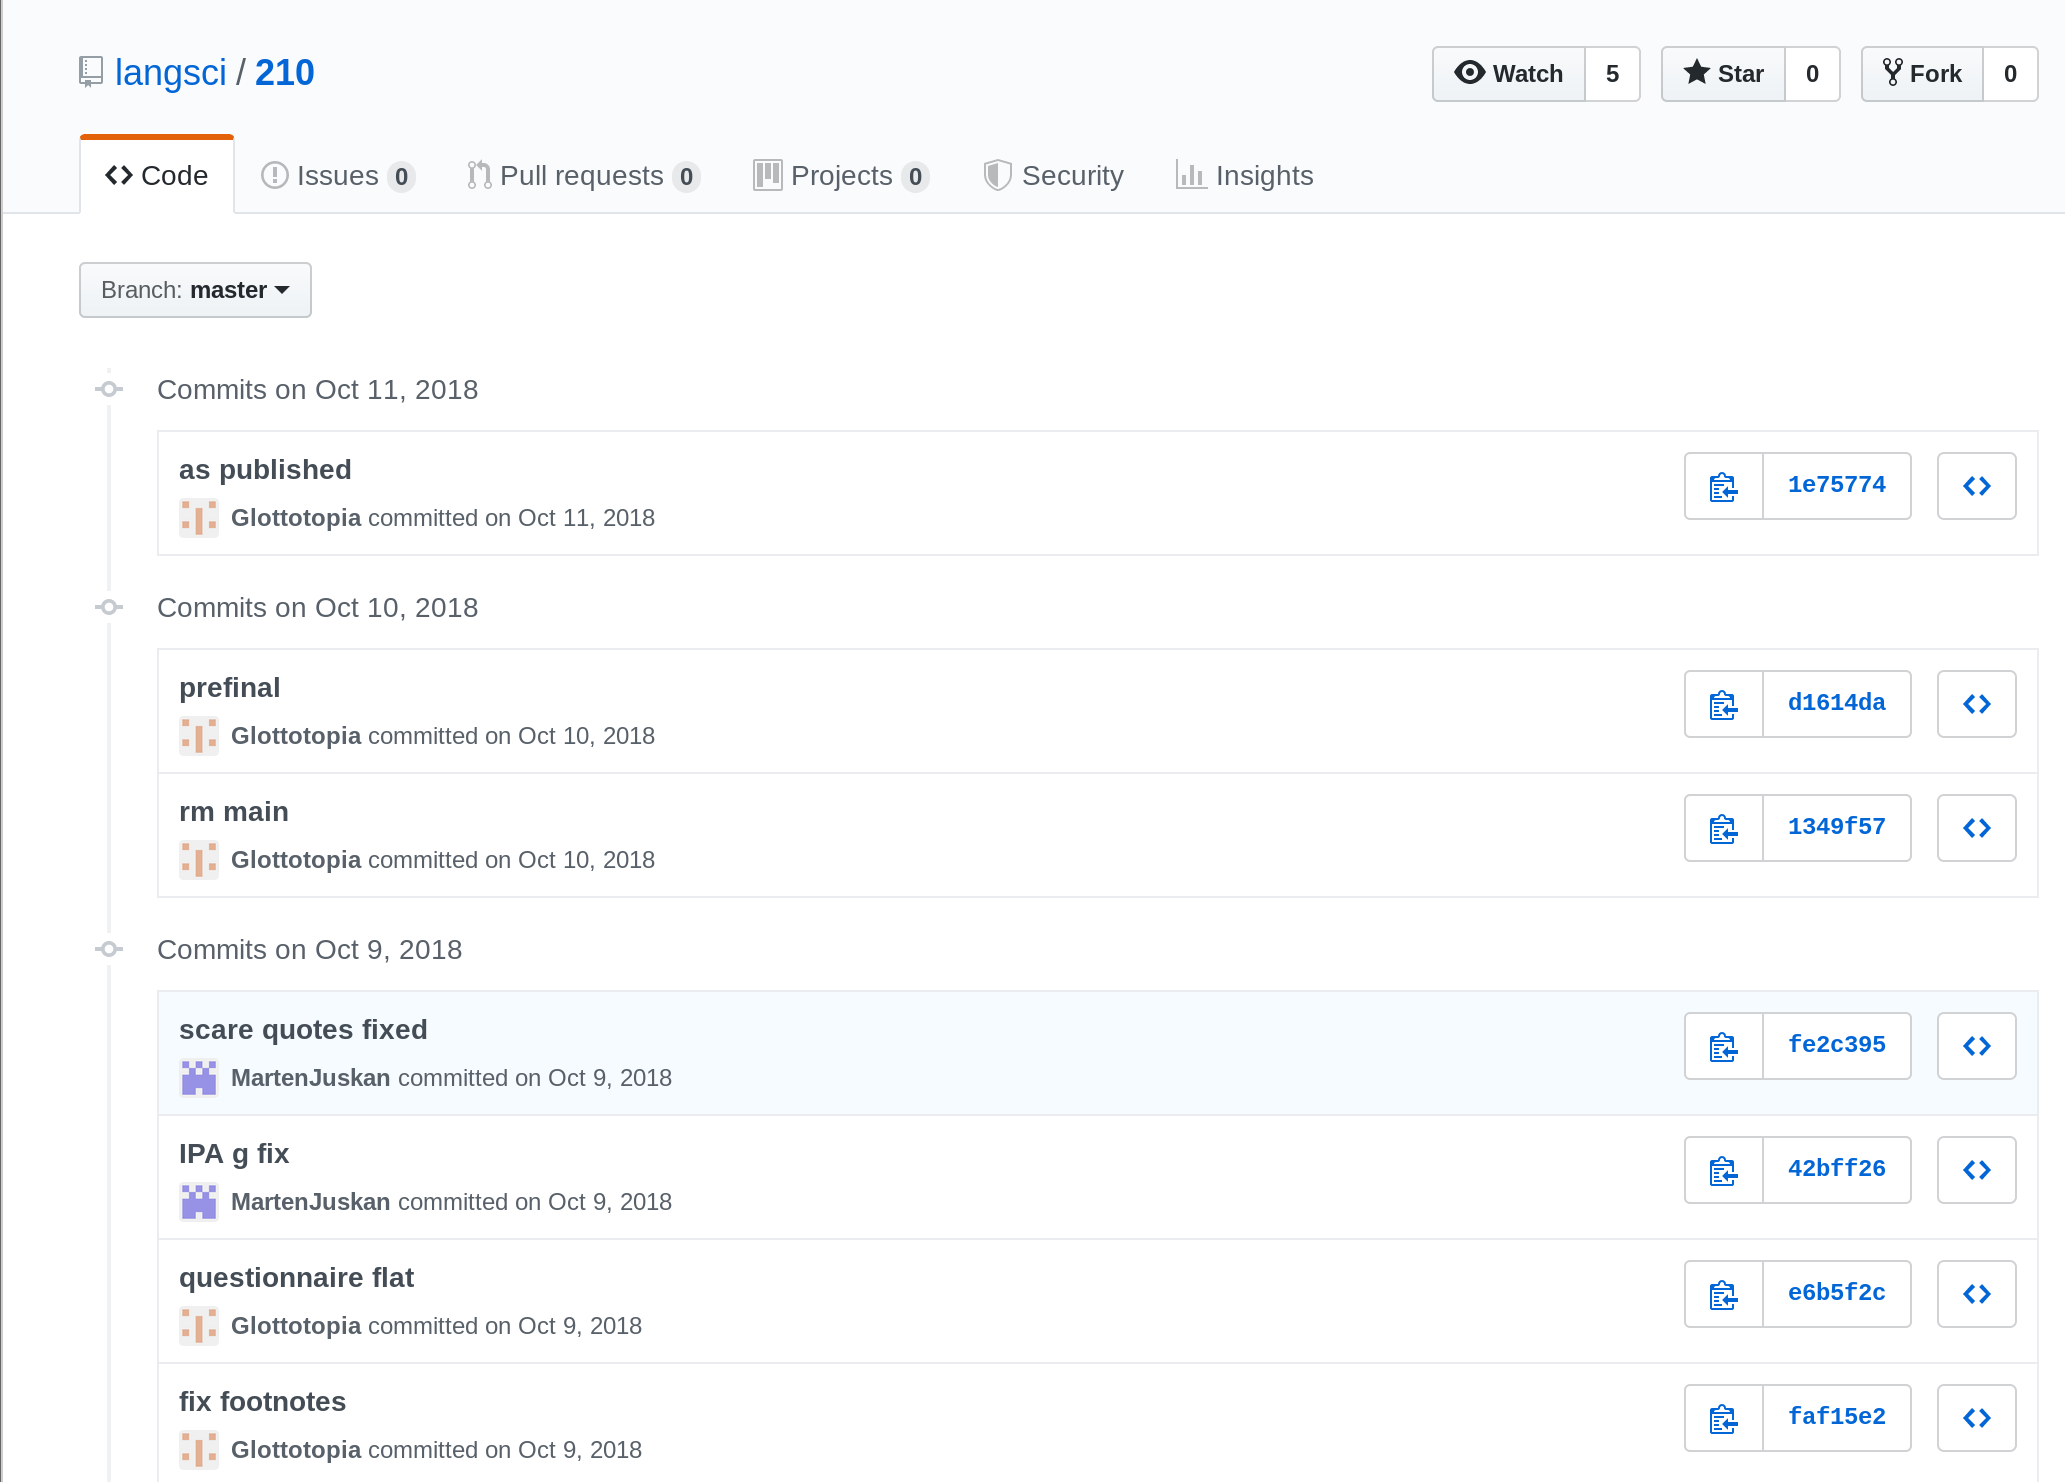
\includegraphics[height=\textheight]{juskancommits.png}
}


\frame{
\frametitle{Versioning: diffs}
  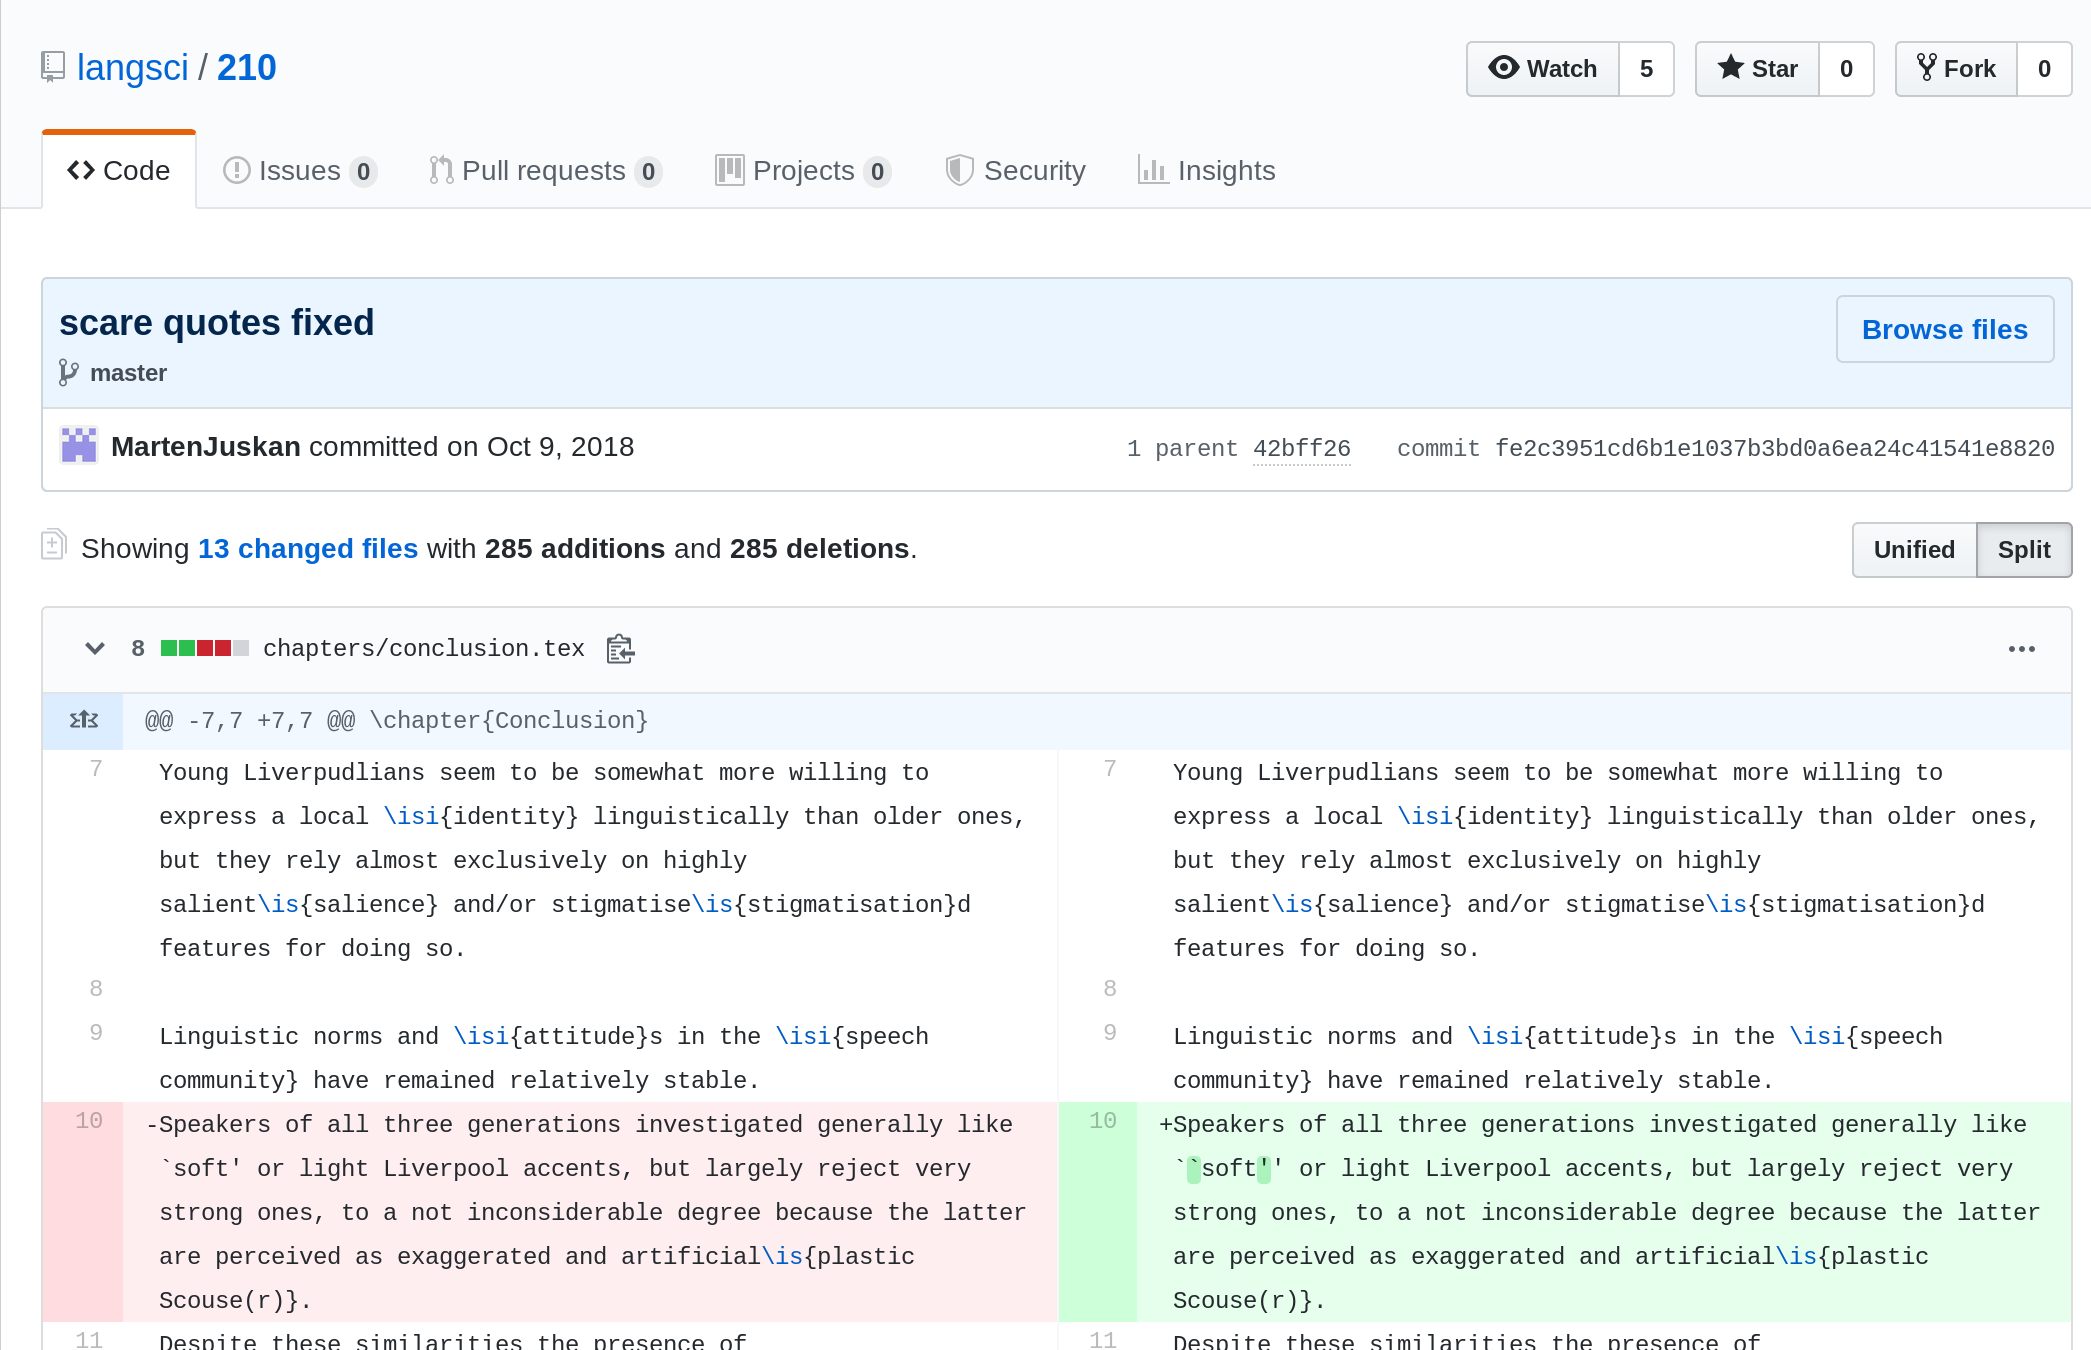
\includegraphics[height=\textheight]{juskansplit.png}
}


\frame{
\frametitle{Versioning: integration}
  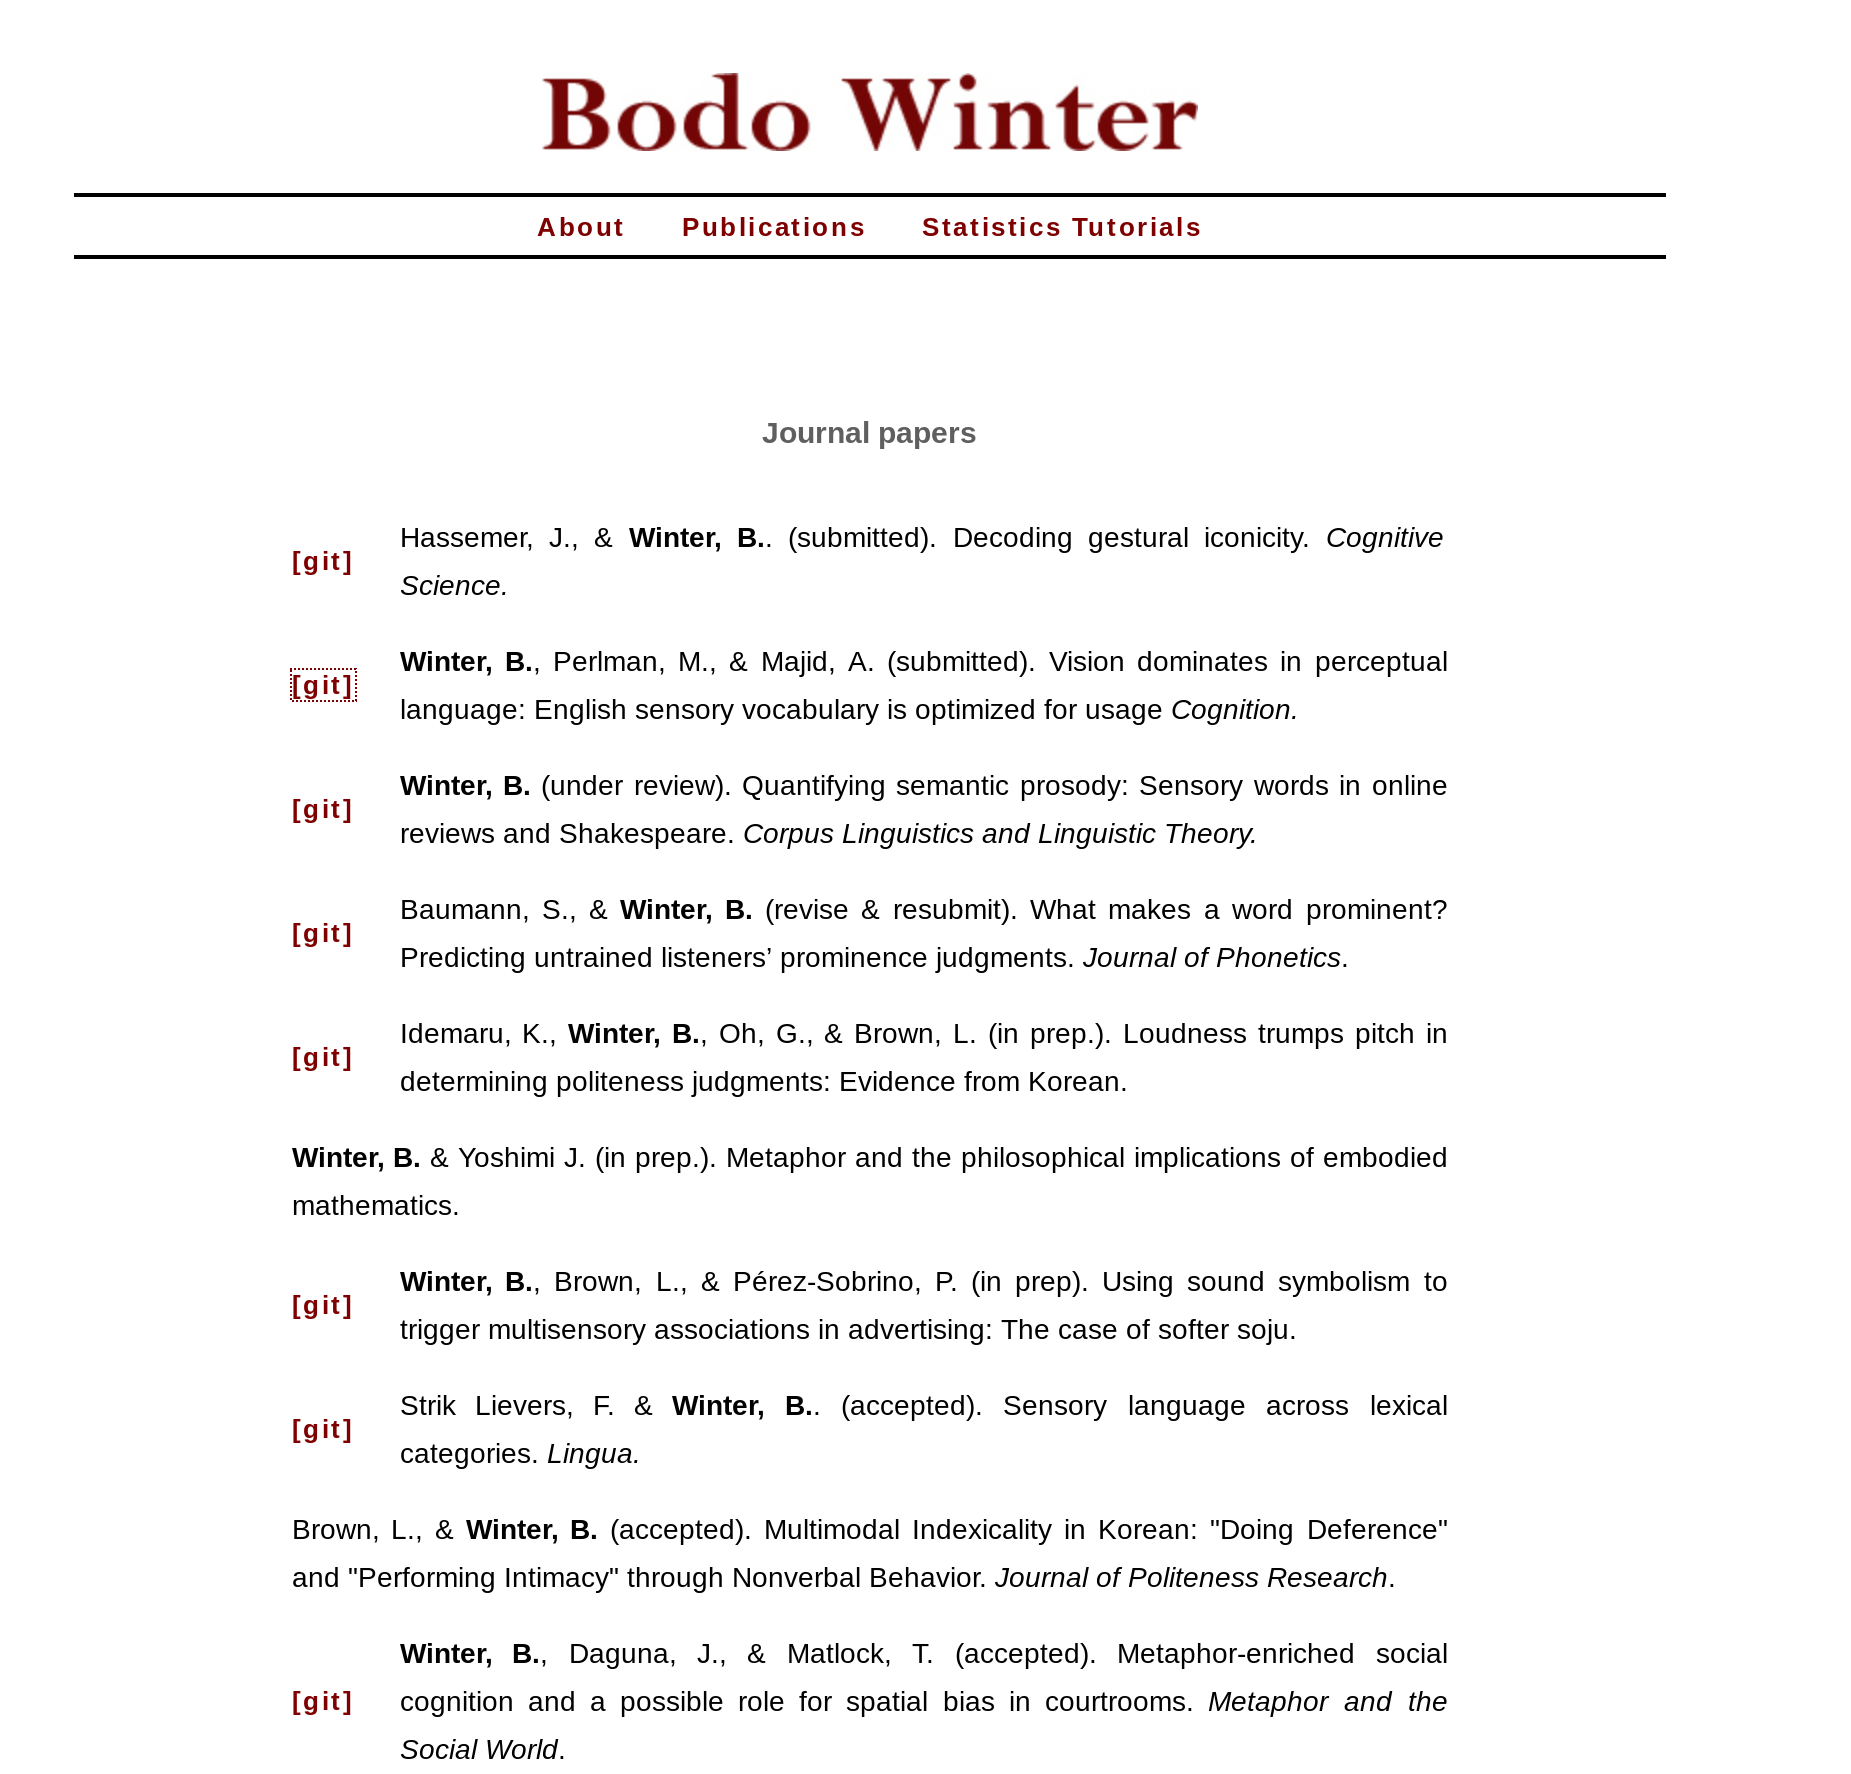
\includegraphics[height=\textheight]{bodowinter.png}
  }

\frame{
\frametitle{GitHub}
   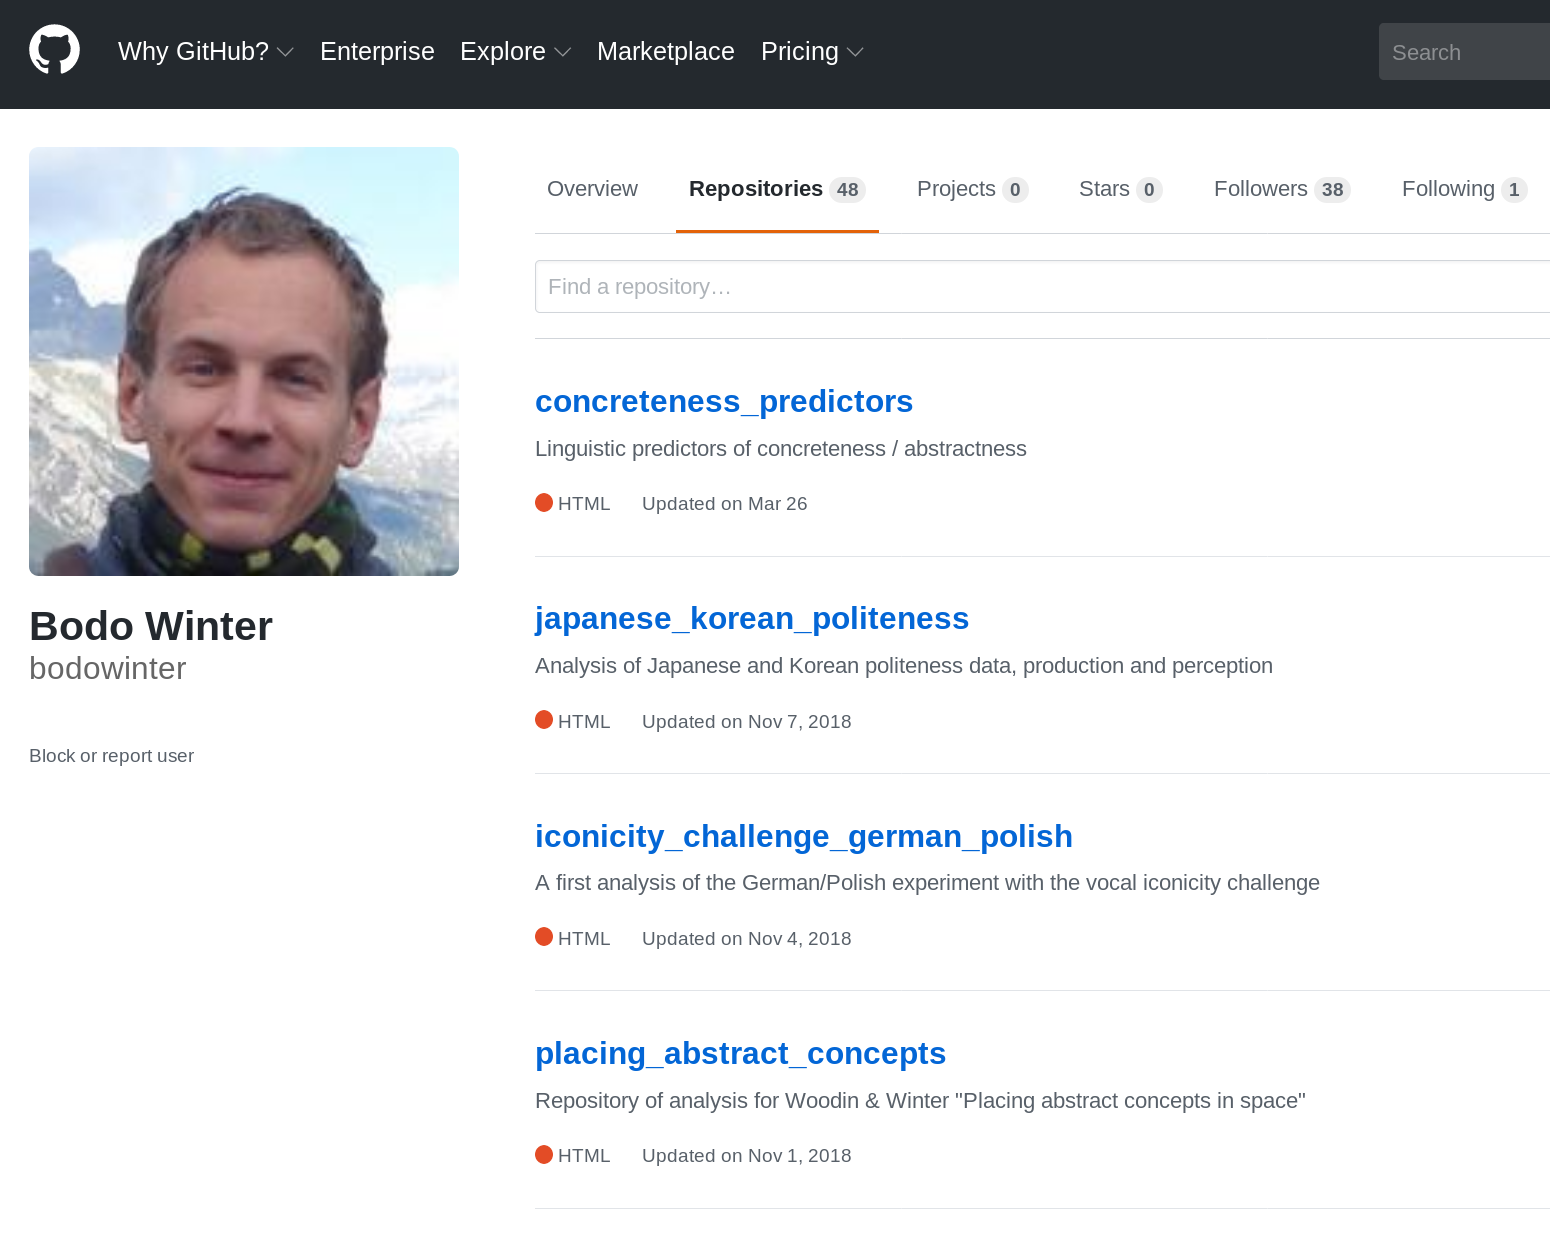
\includegraphics[height=\textheight]{github.png}
}

\frame{
\frametitle{GitHub}
   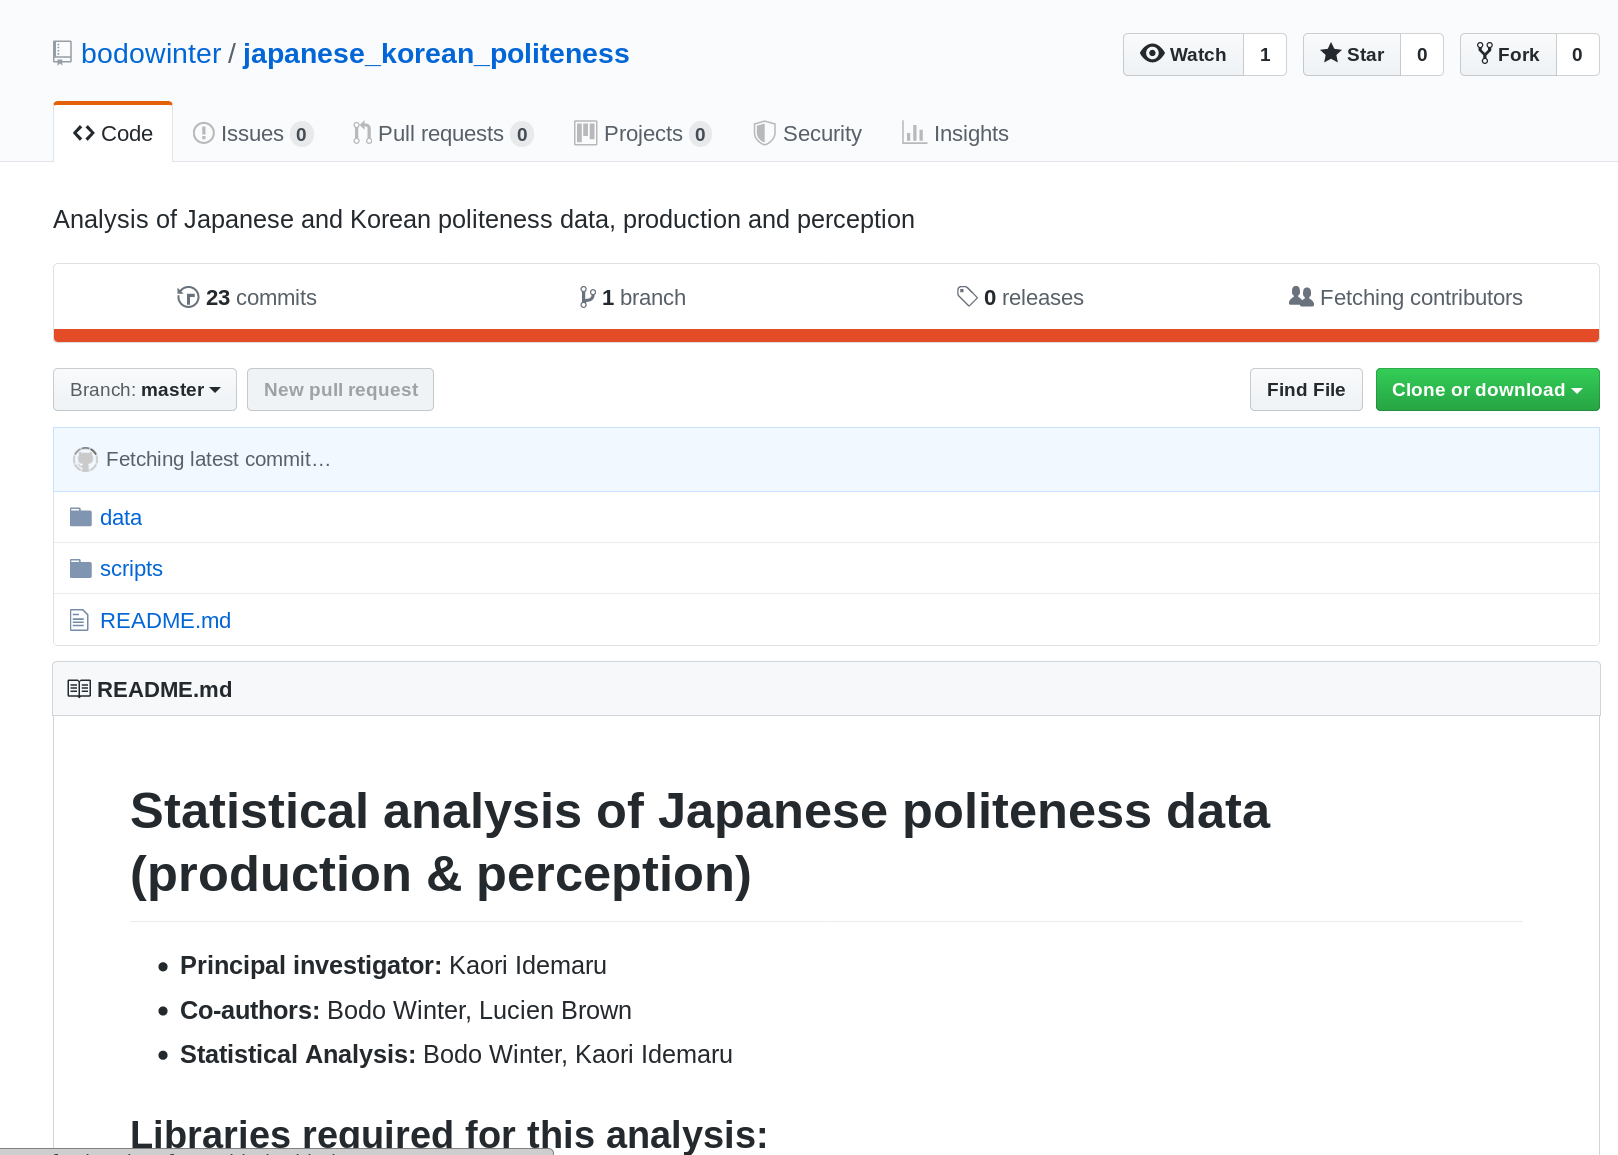
\includegraphics[height=\textheight]{githubjapanese.png}
}

\frame{
\frametitle{Versioning and neat project structure}
\begin{itemize}
  \item Fire-and-forget graphic production is problematic 
  \item adjustments to colours or resolution are not possible anymore at a later point in time. 
\end{itemize}

  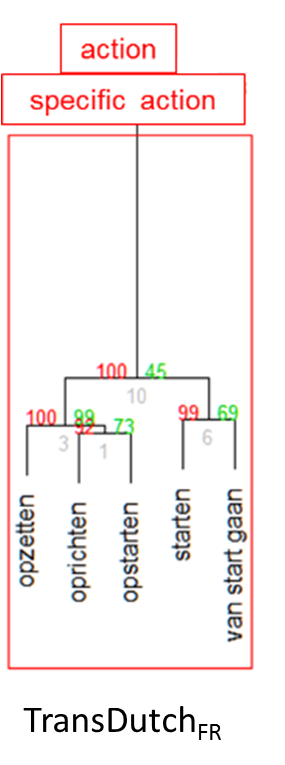
\includegraphics[height=\textheight]{pngR.png}\pause~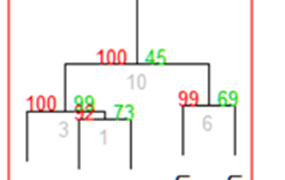
\includegraphics[height=\textheight]{pngR2.png}
}  



\frame{
\frametitle{Versioning and neat project structure}
\begin{columns}
\begin{column}{5cm}
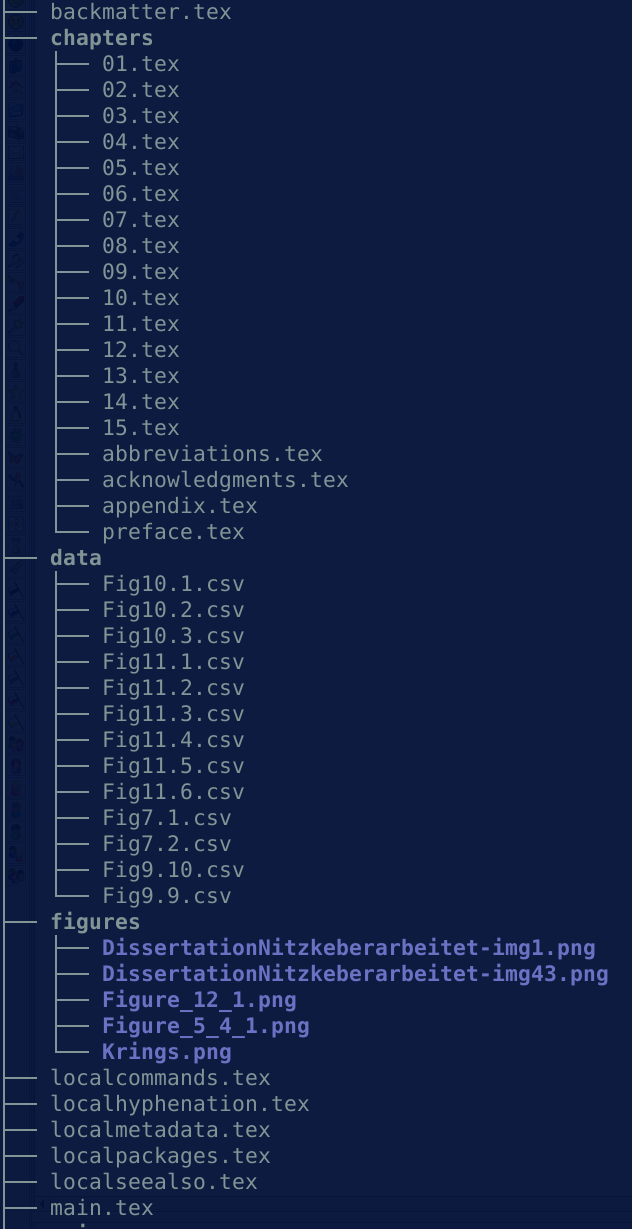
\includegraphics[width=1\textwidth]{folderstructure.png}
\end{column}
\begin{column}{5cm}
\vspace*{-3cm}
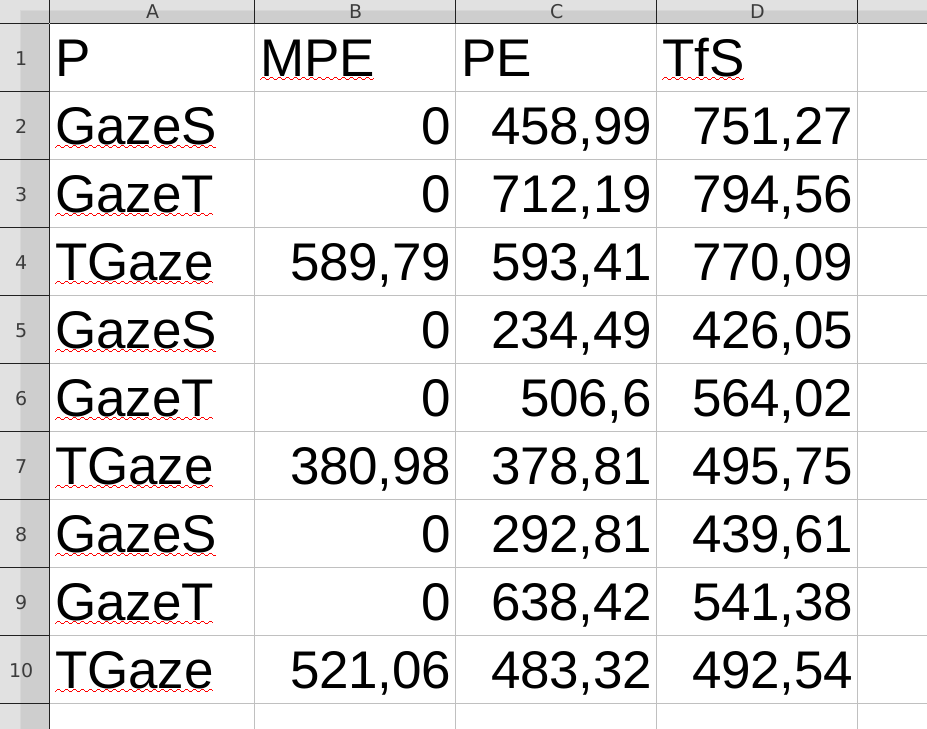
\includegraphics[width=\textwidth]{NitzkecsvLO.png}\\
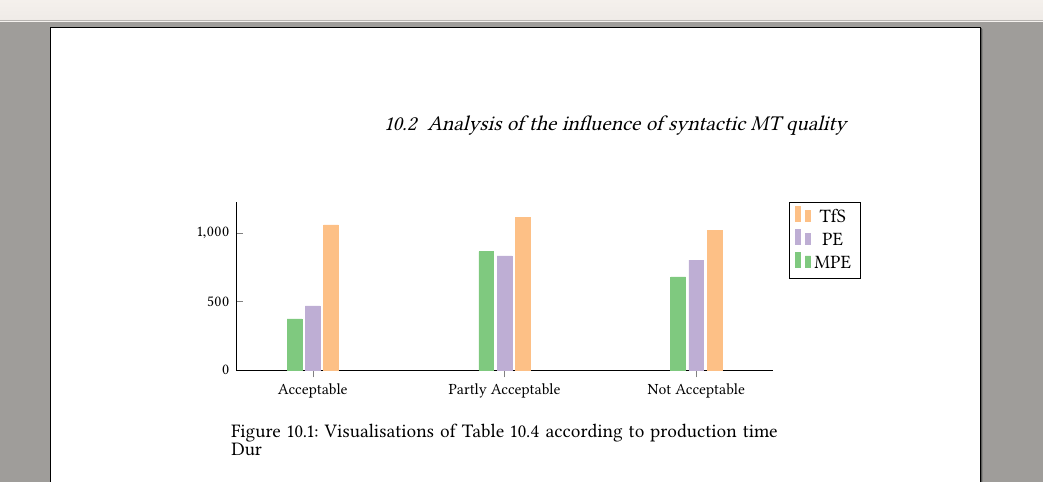
\includegraphics[width=1.2\textwidth]{nitzkebars.png}
\end{column}
\end{columns}
}  



% \frame{
% \frametitle{Versioning: GitHub}
%   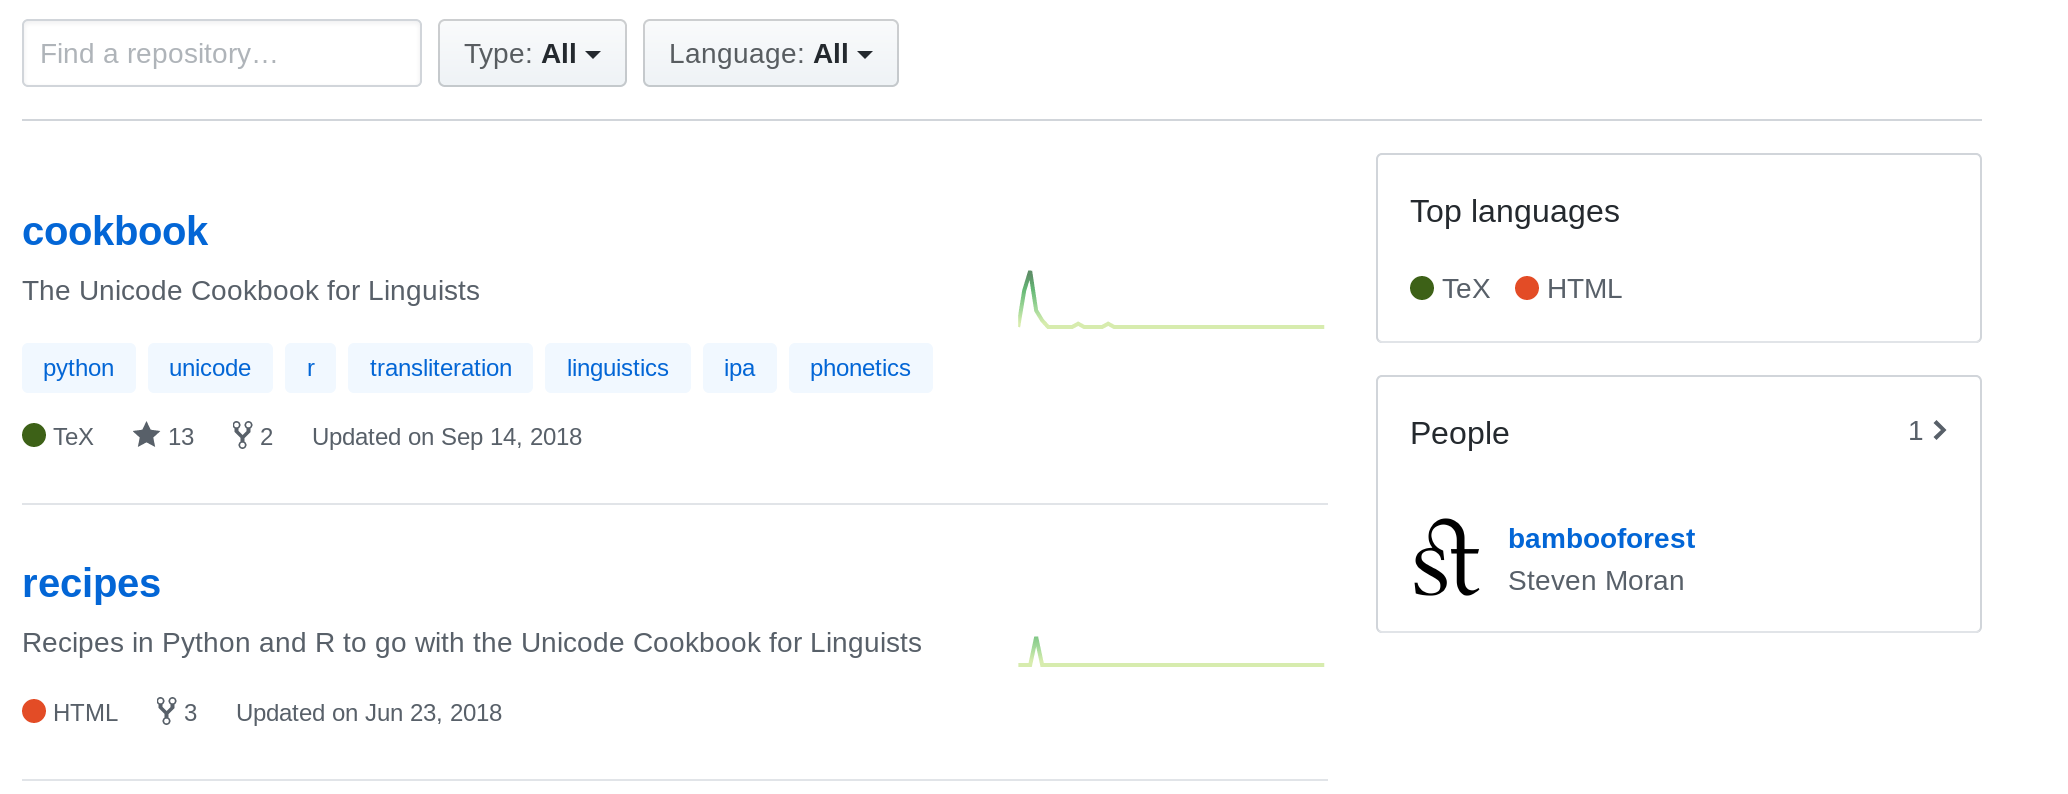
\includegraphics[height=\textheight]{unicodecookbook.png}
% }  
% 
% \frame{
% \frametitle{Versioning: releases}
%   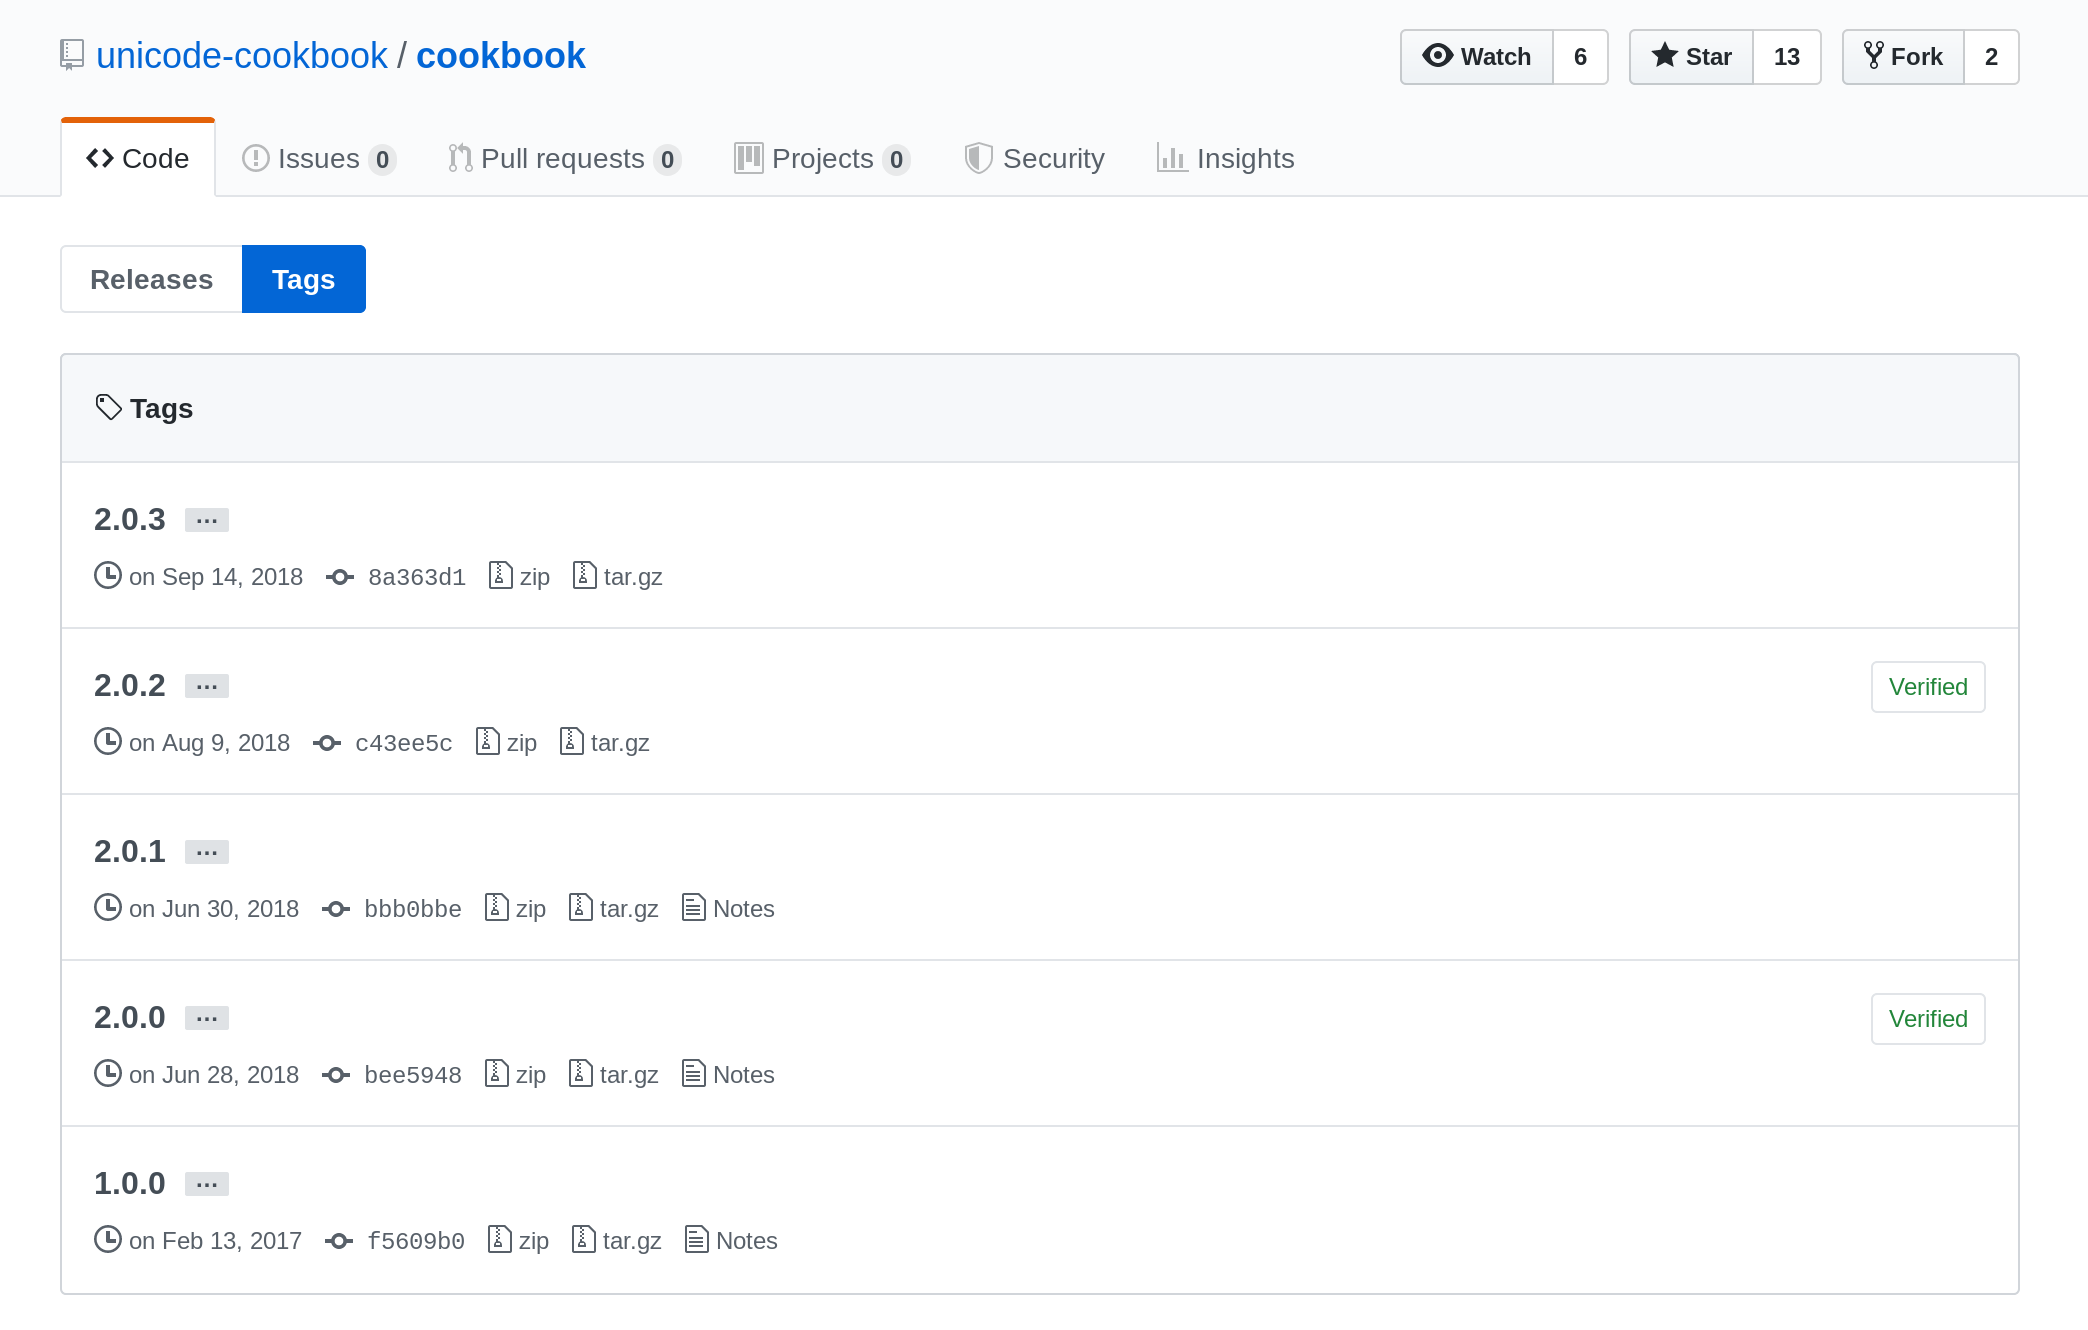
\includegraphics[height=\textheight]{releases.png}
% }  


\frame{
\frametitle{Repositories}
%   \includegraphics[height=.2\textheight]{./path/to/graphicsfile}
  \begin{itemize}
    \item Repositories collect documents and research data 
      \begin{itemize}
        \item \textbf{discipline-specific} or \textbf{general purpose}
        \item \textbf{preprint} or \textbf{postprint} 
        \item \textbf{text} or \textbf{data} 
      \end{itemize}
  \end{itemize}
}

\frame{
\frametitle{figshare}
   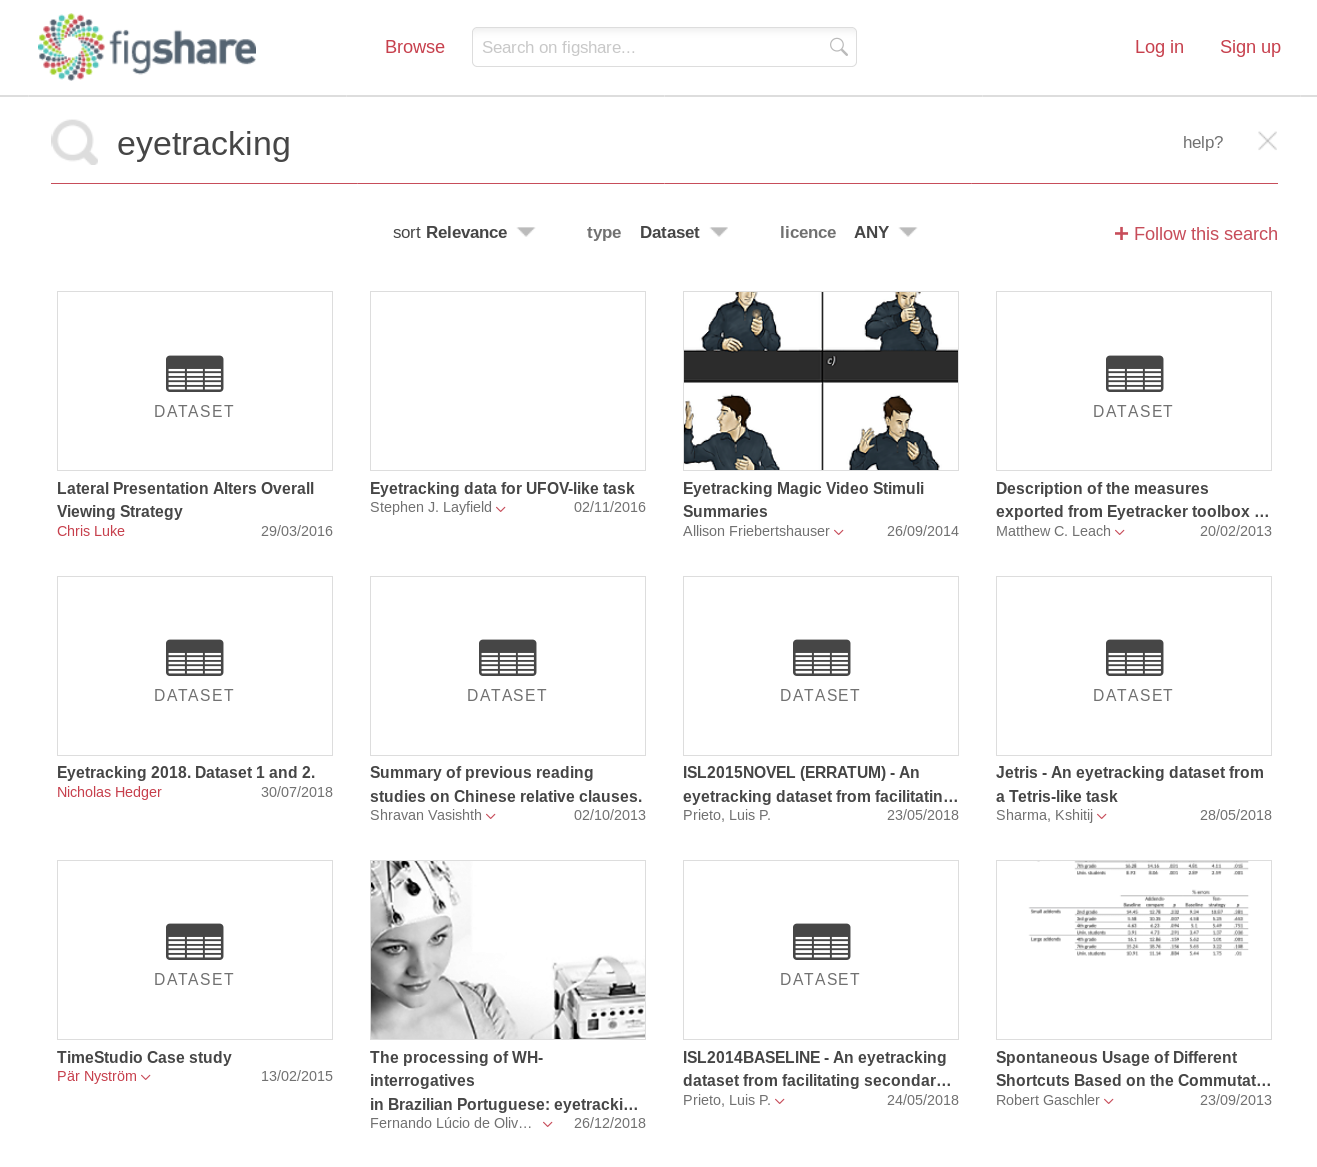
\includegraphics[height=\textheight]{figshare.png}
}

% \frame{
%    \includegraphics[height=\textheight]{dryad.png}
% }

\frame{
\frametitle{Trolling}
   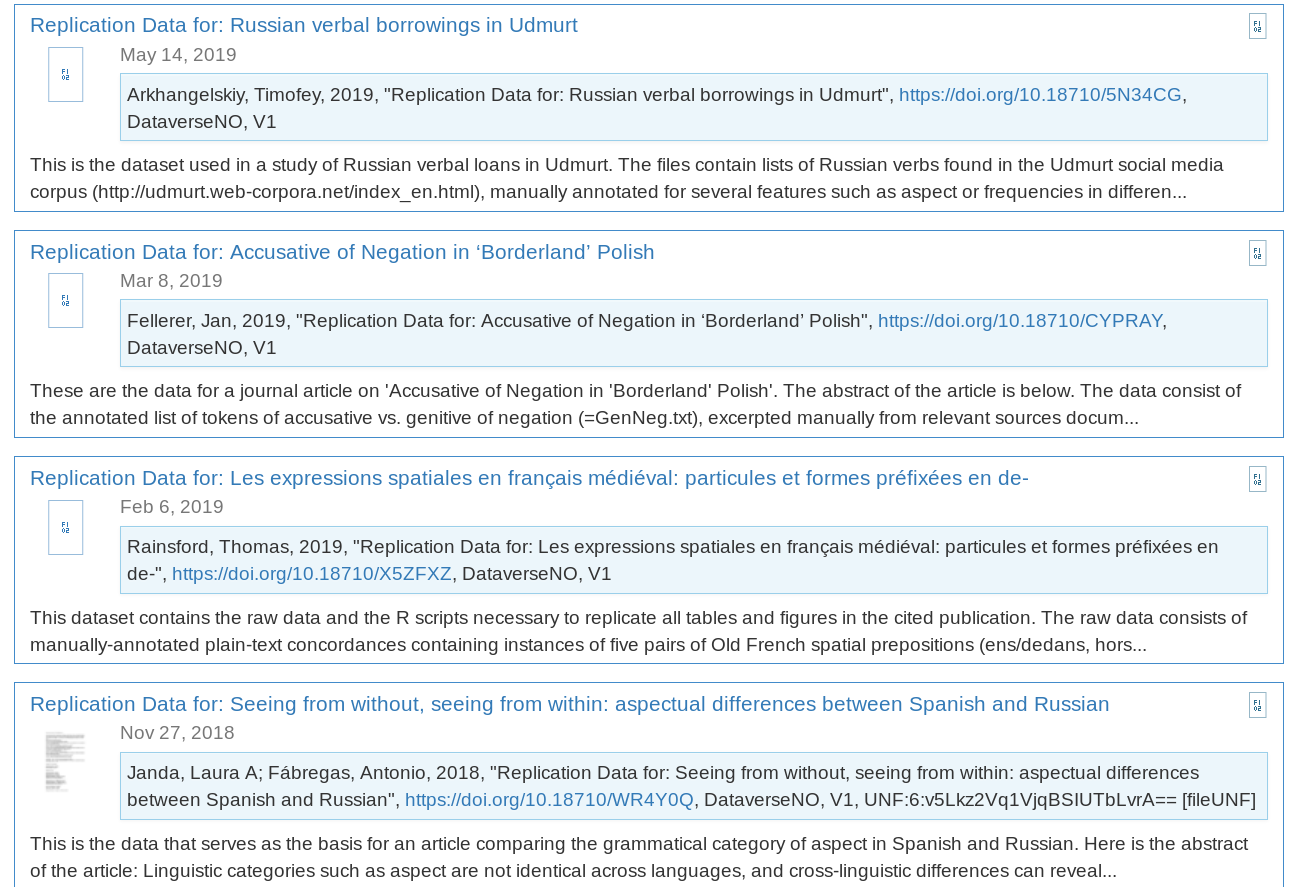
\includegraphics[height=\textheight]{trolling.png}
}

\frame{
\frametitle{LingBuzz}
   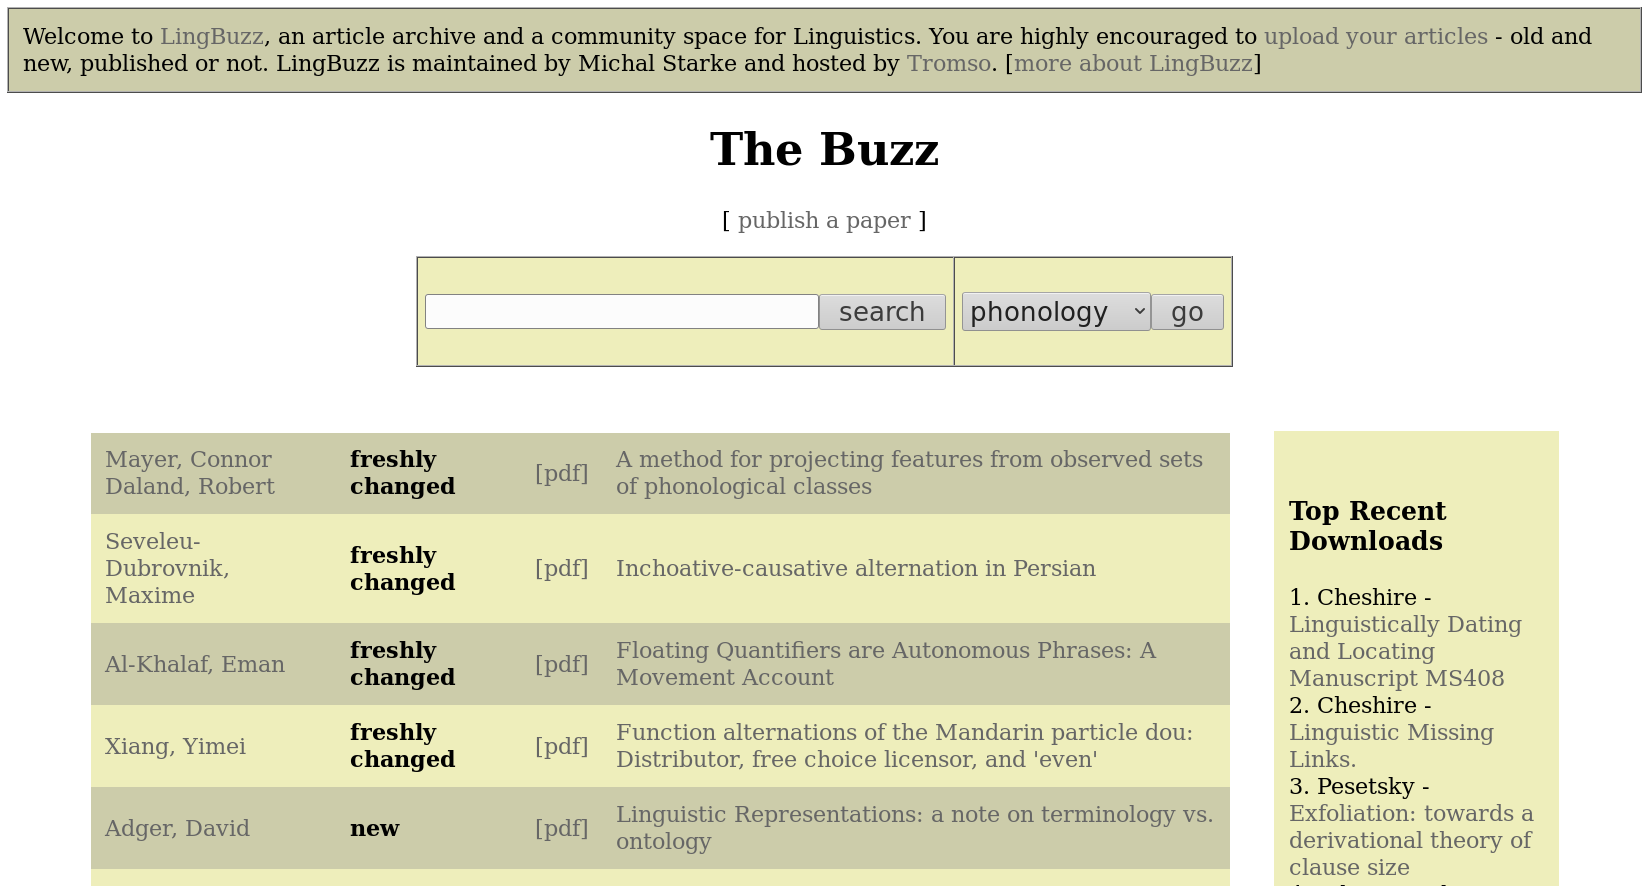
\includegraphics[height=\textheight]{lingbuzz.png}
}

\frame{
\frametitle{semanticsarchive.net}
   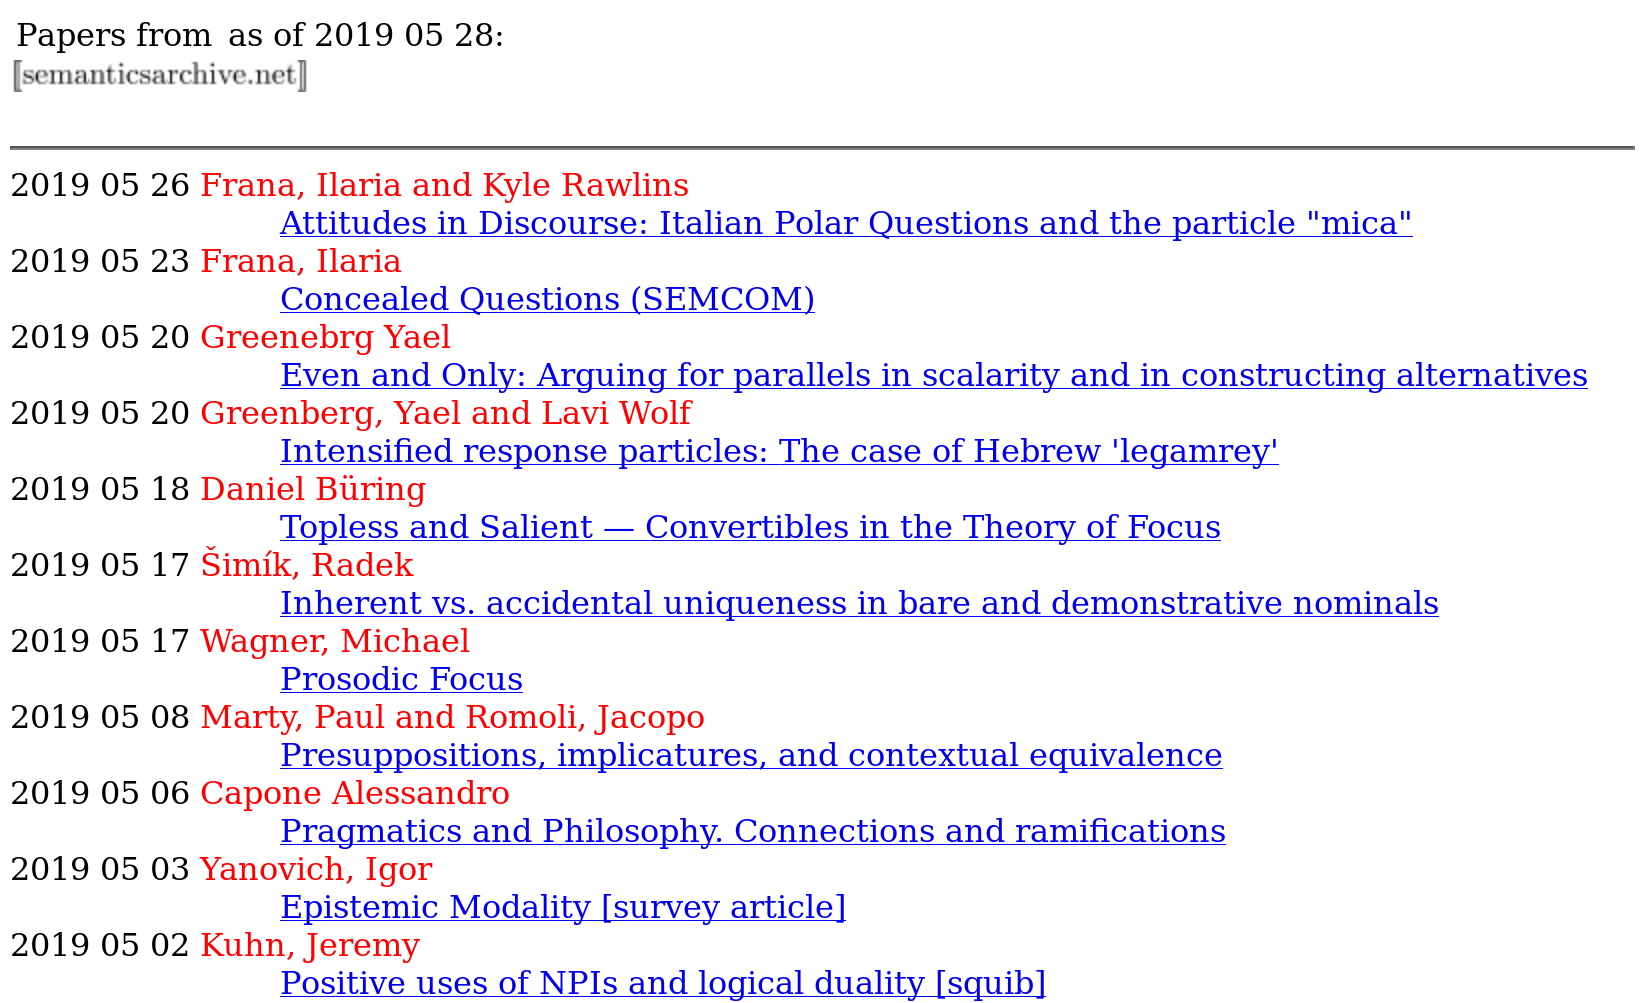
\includegraphics[height=\textheight]{semanticsarchive.png}
}

% \frame{
% \frametitle{Rutgers Optimality Archive}
%    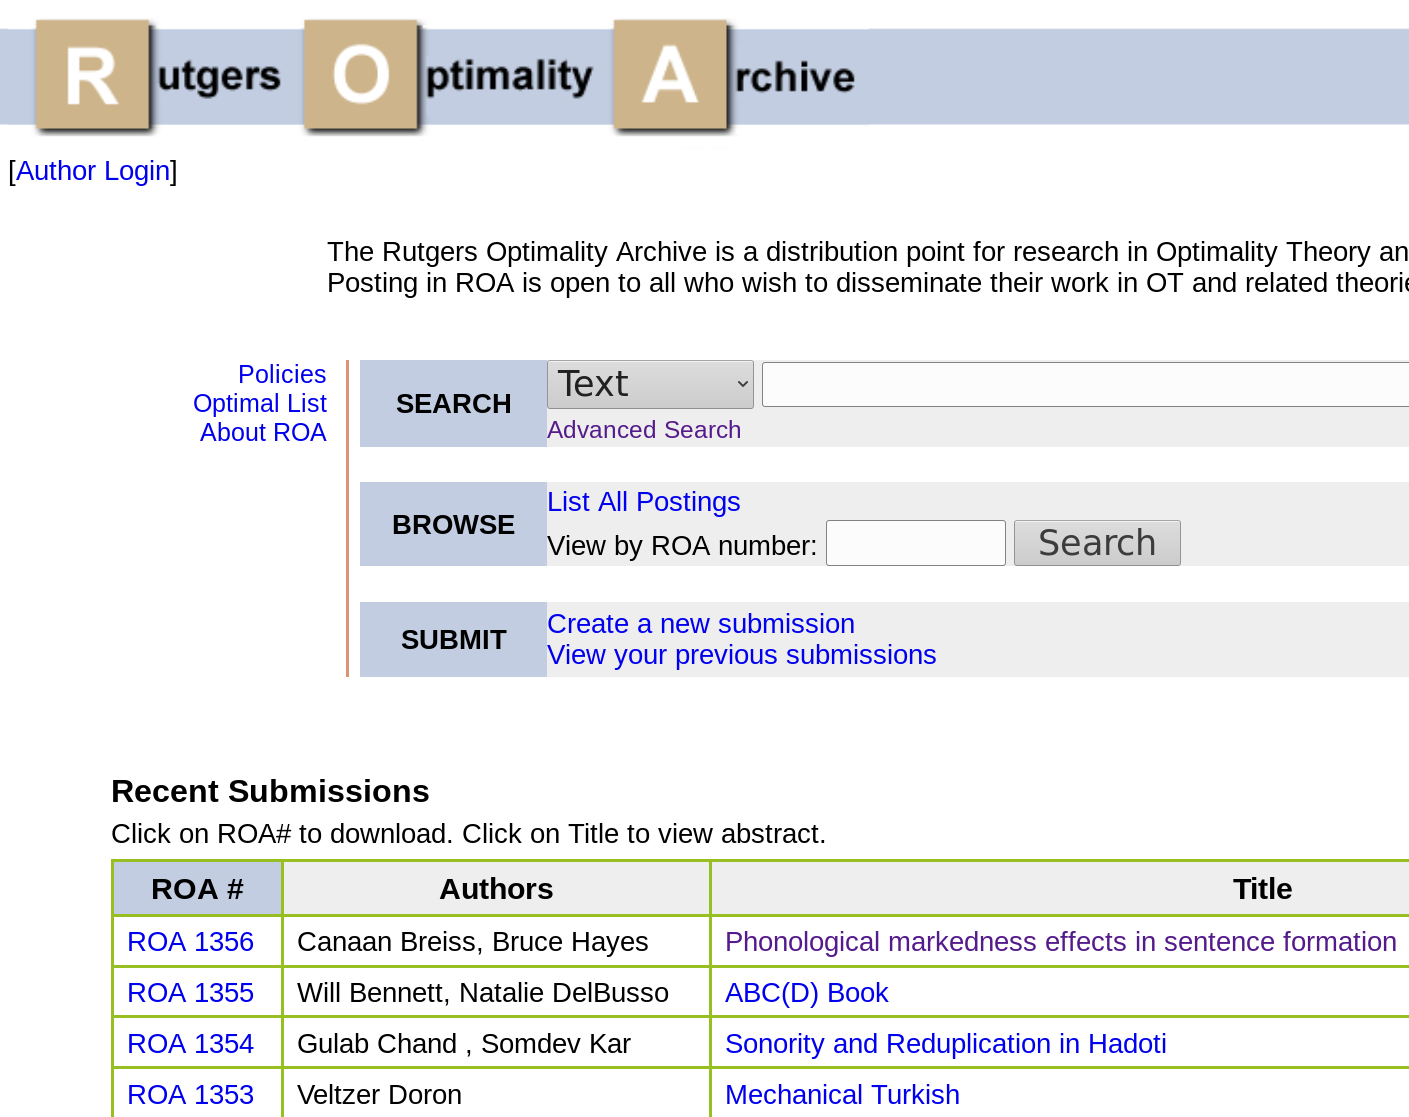
\includegraphics[height=\textheight]{roa.png}
% }


\frame{
\frametitle{Endangered Languages\\ Archive}
   
\includegraphics[height=\textheight]{elar.png}
}


\frame{
\frametitle{Zenodo}
   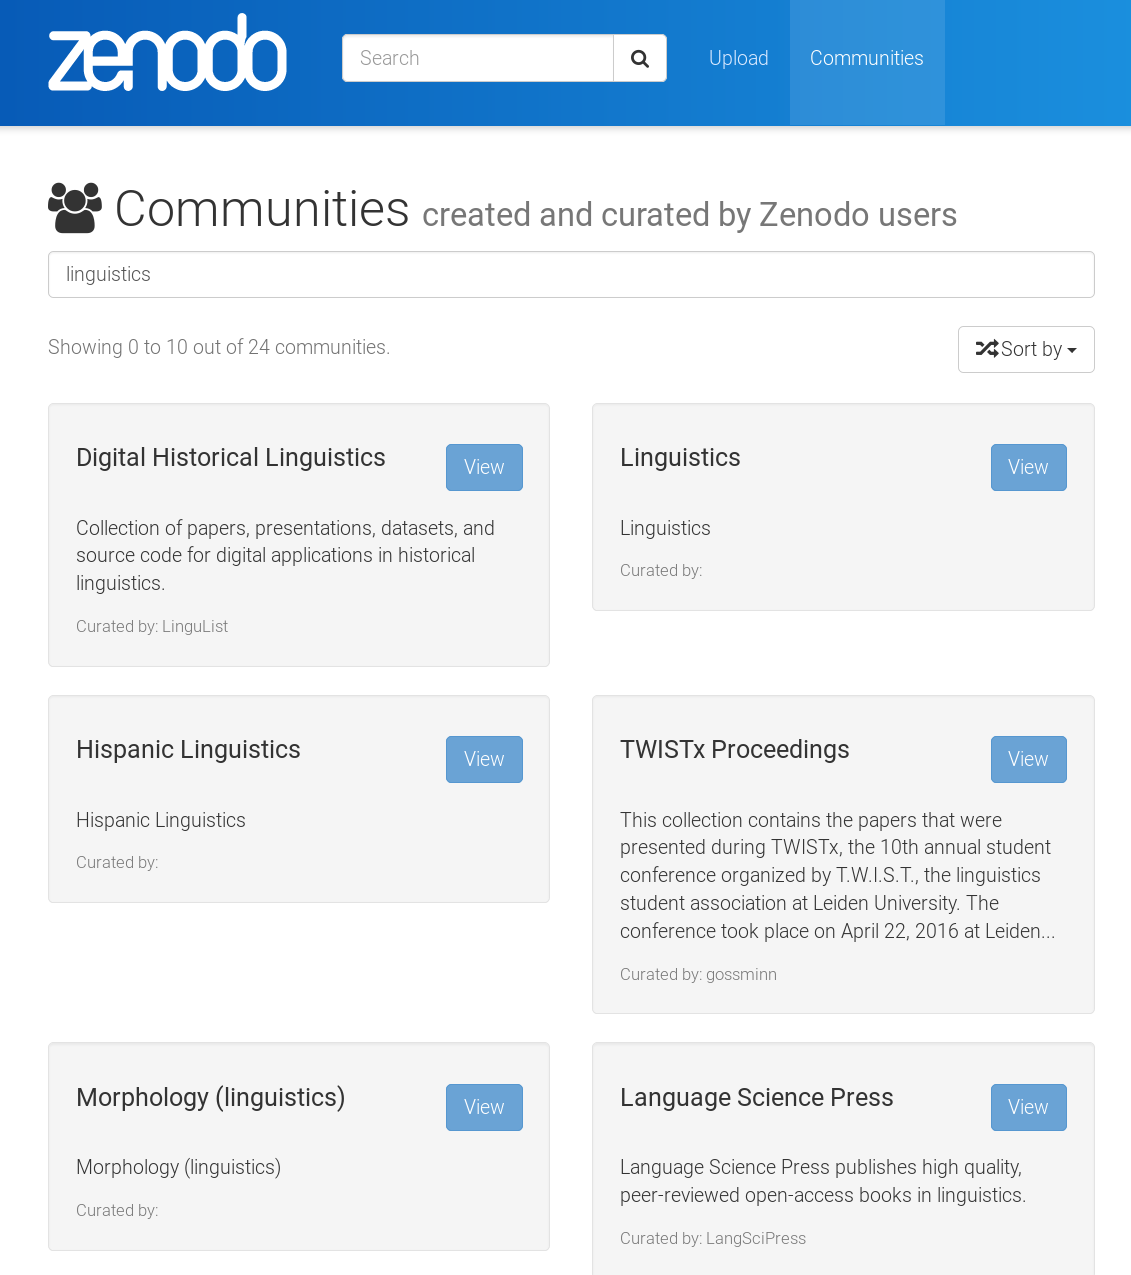
\includegraphics[height=\textheight]{zenodo.png}
}



\frame{
\frametitle{Academia and Researchgate}
  \begin{itemize}
    \item  Academia.edu and researchgate are NOT repositories
    \item both make money from restricting access
    \end{itemize}
}                    

\frame{
\frametitle{A note on scooping}
  \begin{itemize}
    \item  Scooping means that someone ``steals'' your research while you are still finalising it
    \item that fear is by and large unwarranted 
    \item you can count yourself happy if anybody IS actually interested in your data!
    \item most research actually struggles a lot more with a lack of interest to outsiders rather than scooping 
    \item preprint servers allow you to register your data and establish primacy
  \end{itemize}
}
            

\frame{
\frametitle{Recommendations for\\ technical sustainability}
  \begin{itemize}
  \highlight
    \item conceptually separate your data, code, and prose text   
    \item make sure you can replicate all steps of your analysis
    \item ideally, specify automated pipelines for your analysis
    \item do not hardwire data and code
    \item use a citation manager 
    \item use a versioning tool 
    \begin{itemize}\highlight
      \item local or university or cloud
    \end{itemize}
    \item use a preprint server
    \item backup\pause
    \item backup\pause
    \item backup
    \end{itemize}
%   \color{black}\normalfont
}


            
\section{Legal aspects}

\frame{
\frametitle{Legal sustainability}
  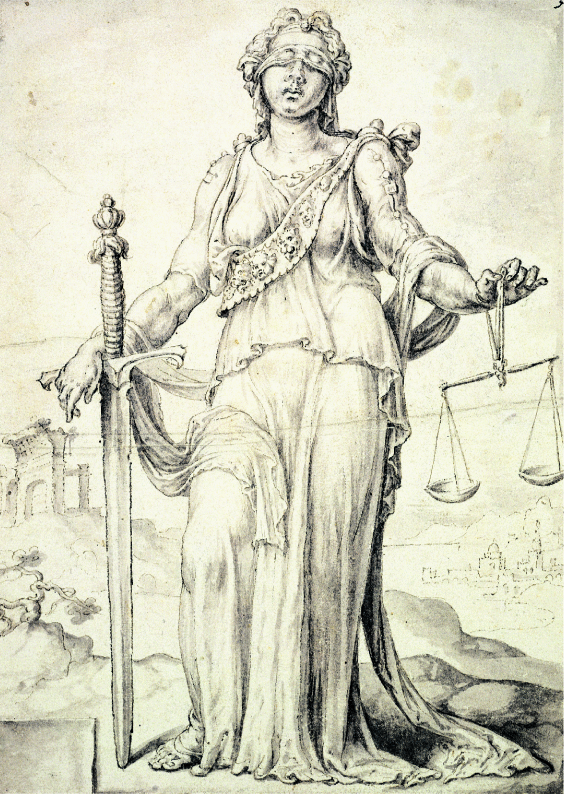
\includegraphics[height=\textheight]{justitia.png}
}

\frame{
\frametitle{Intellectual Property Rights}
%   \includegraphics[height=.2\textheight]{./path/to/graphicsfile}
  \begin{itemize}
    \item  ``Copyright'' in the Anglo-Saxon countries
    \item  ``Urheberrecht'' in continental Europe 
    \item These are different!
    \item Once you create somehting, you can decide who can use it and how
    \item Choose wisely and be explicit!
  \end{itemize}
}

\frame{
\frametitle{License}
%   \includegraphics[height=.2\textheight]{./path/to/graphicsfile}
  \begin{itemize}
    \item  Usage rights can be differentiated as follows
    \begin{itemize}
      \item geographical restriction (e.g. \textit{only for Germany})
      \item type restrictions (e.g. \textit{only for print}) 
      \item exclusive (no-one else has the right) vs. non-exclusive (other people may also get the rights)
      \item copyright transfer agreement (Anglo-Saxon culture)
      \item total buy-out
    \end{itemize}
  \end{itemize}
}

\frame{
\frametitle{Copyright transfer agreement}

\includegraphics[width=\textwidth]{copyrighttransfer.pdf}
}

\frame{
\frametitle{Contracts}
%   \includegraphics[height=.2\textheight]{./path/to/graphicsfile}
  \begin{itemize}
    \item  Publisher contracts restrict everybody, including yourself 
    \item once you sign away your copyright, you have no longer the right to use your own material 
    \item to reuse tables or graphics in subsequent works of yours, you must first ask the new rights holder for permission 
    \item chasing rights is incredibly annoying
    \item publishers will put your content behind a paywall, meaning that it can actually be more difficult to access once it is officially published than before
    \item publisher vary as to whether and when they allow books to be hosted in repositories  
  \end{itemize}
    }

\frame{
\frametitle{Availability of Nordhoff (ed.) (2012)}
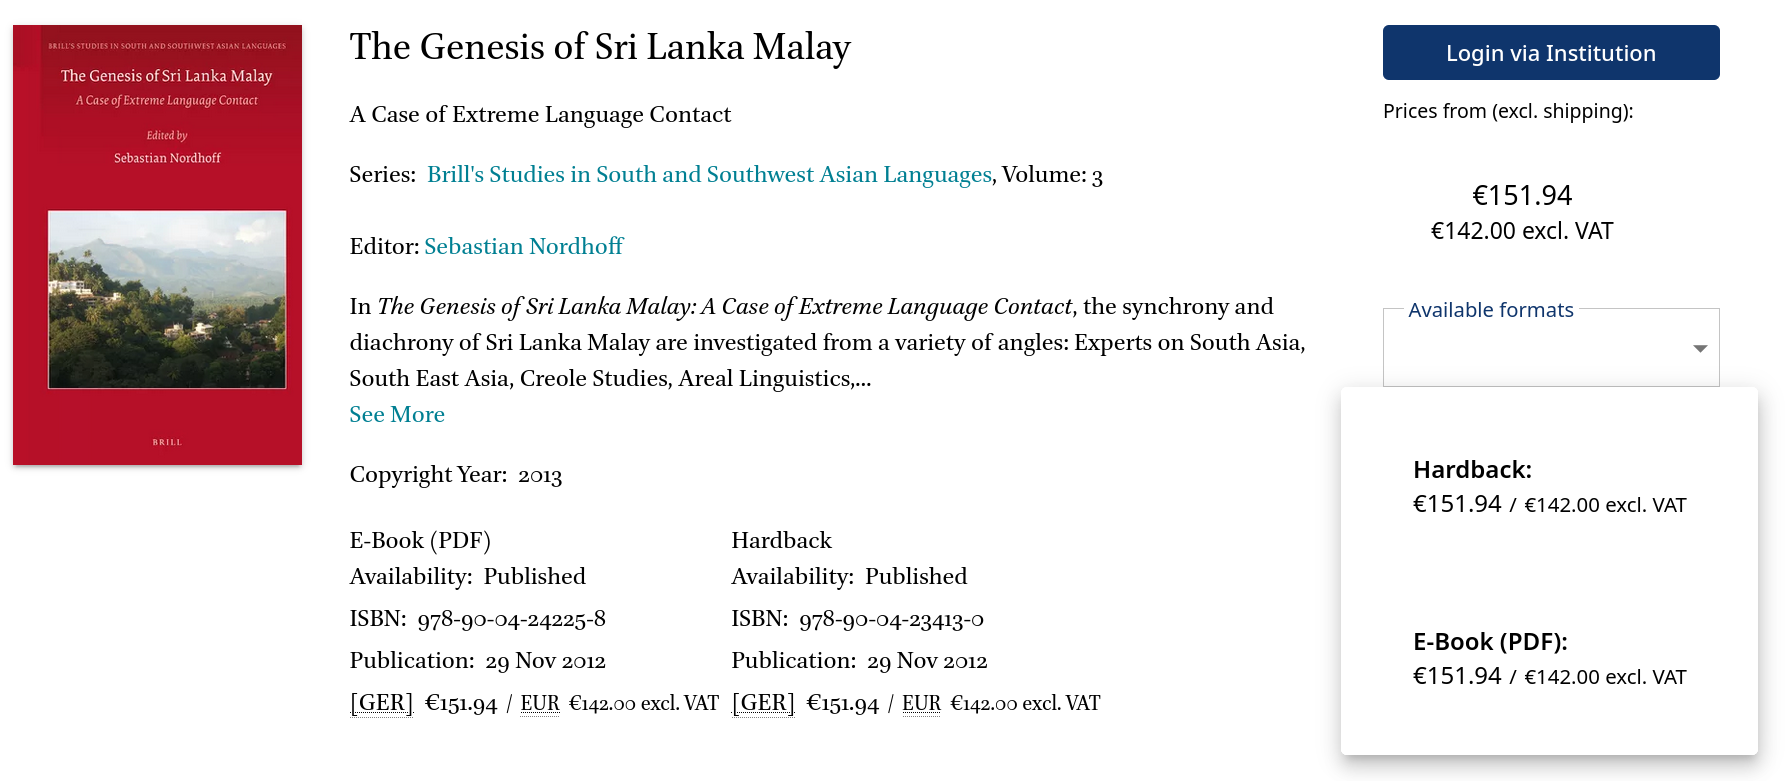
\includegraphics[width=\textwidth]{brillnordhoff.png}
 }

\frame{ 
\frametitle{Recommendations for legal sustainability}
  \begin{itemize}
  \highlight
    \item Publish your works under a Creative Commons license, preferably CC-BY 
    \begin{itemize}\highlight
      \item see the Berlin|Budapest|Bethesda declarations on Open Access 
    \end{itemize}
    \item This license clearly states who the copyright holder is and how the content can be reused (typically requiring only the attribution of the original author)
    \item see Fair Open Access principles on \url{https://www.lingoa.eu/about/mission}
    \item do not sign away your copyright \pause
    \item do not sign away your copyright \pause 
    \item do not sign away your copyright
  \end{itemize}
}
                
%                 The editor hereby assigns to the Publisher the full copyright in the Work [...]. Consequently, the Publisher shall have the exclusive right \textbf{throughout the world} to publish and sell th Work in \textbf{all languages}, in whole or in part, including, \textbf{without limitation}, \textbf{any} abridgement and substantial part thereof, in book form and in \textbf{any other form} including, without limitation, mechanical, digital electronic, and visual reproduction, electronic storage and retrieval systems, including internet and intranet delivery and \textbf{all other forms of electronic publication now known or hereinafter invented}. 
                
\section{Financial aspects}
\frame{
\frametitle{Financial aspects of\\ sustainability}
  
\includegraphics[height=\textheight]{calculation.jpg}
 {\tiny CC-BY-ND Dennis Skley \url{https://www.flickr.com/photos/dskley/14895278831}}
 }
 
\frame{
\frametitle{Print run}
%   \includegraphics[height=.2\textheight]{./path/to/graphicsfile}
  \begin{itemize}
    \item  How many books does a publisher print? 
  \end{itemize}
} 

\frame{
\frametitle{Cost for printing one book per Print-on-Demand}

\includegraphics[width=\textwidth]{printingcosts.png}
}

\frame{
\frametitle{Print run}
%   \includegraphics[height=.2\textheight]{./path/to/graphicsfile}
  \begin{itemize}
    \item  How many books does a publisher sell?
    \item How much does the author typically earn?
  \end{itemize}
} 

\frame{
  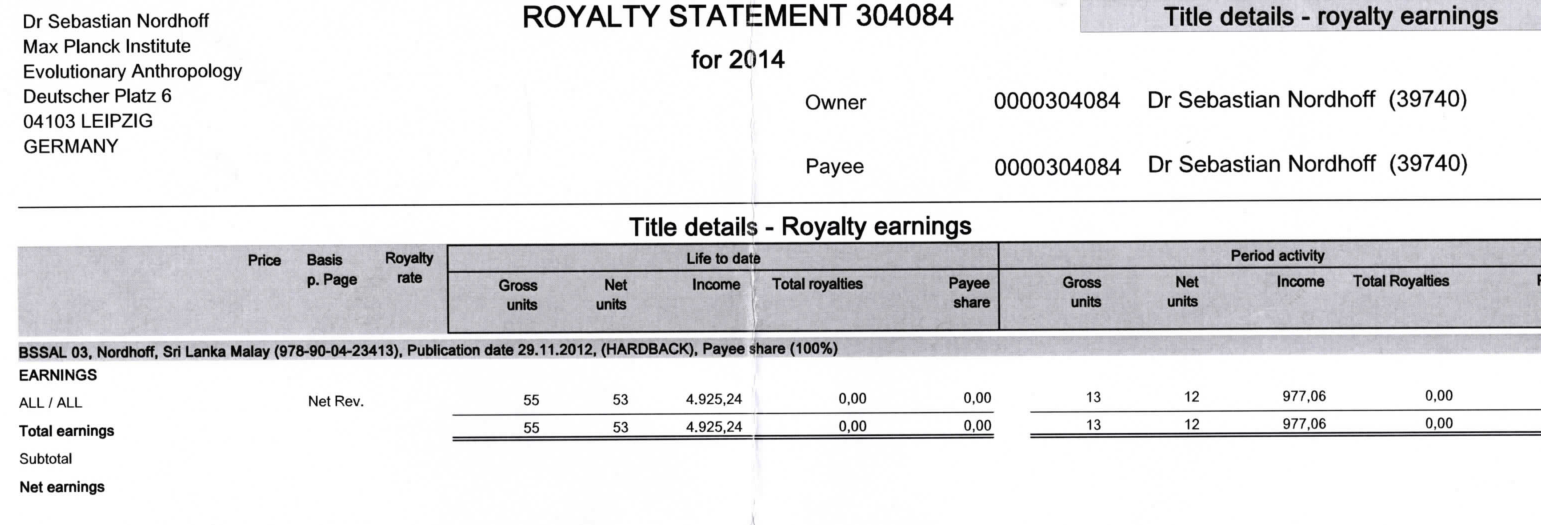
\includegraphics[width=\textwidth]{royalty.pdf}
}        

\frame{
\frametitle{Funding models: reader pays}
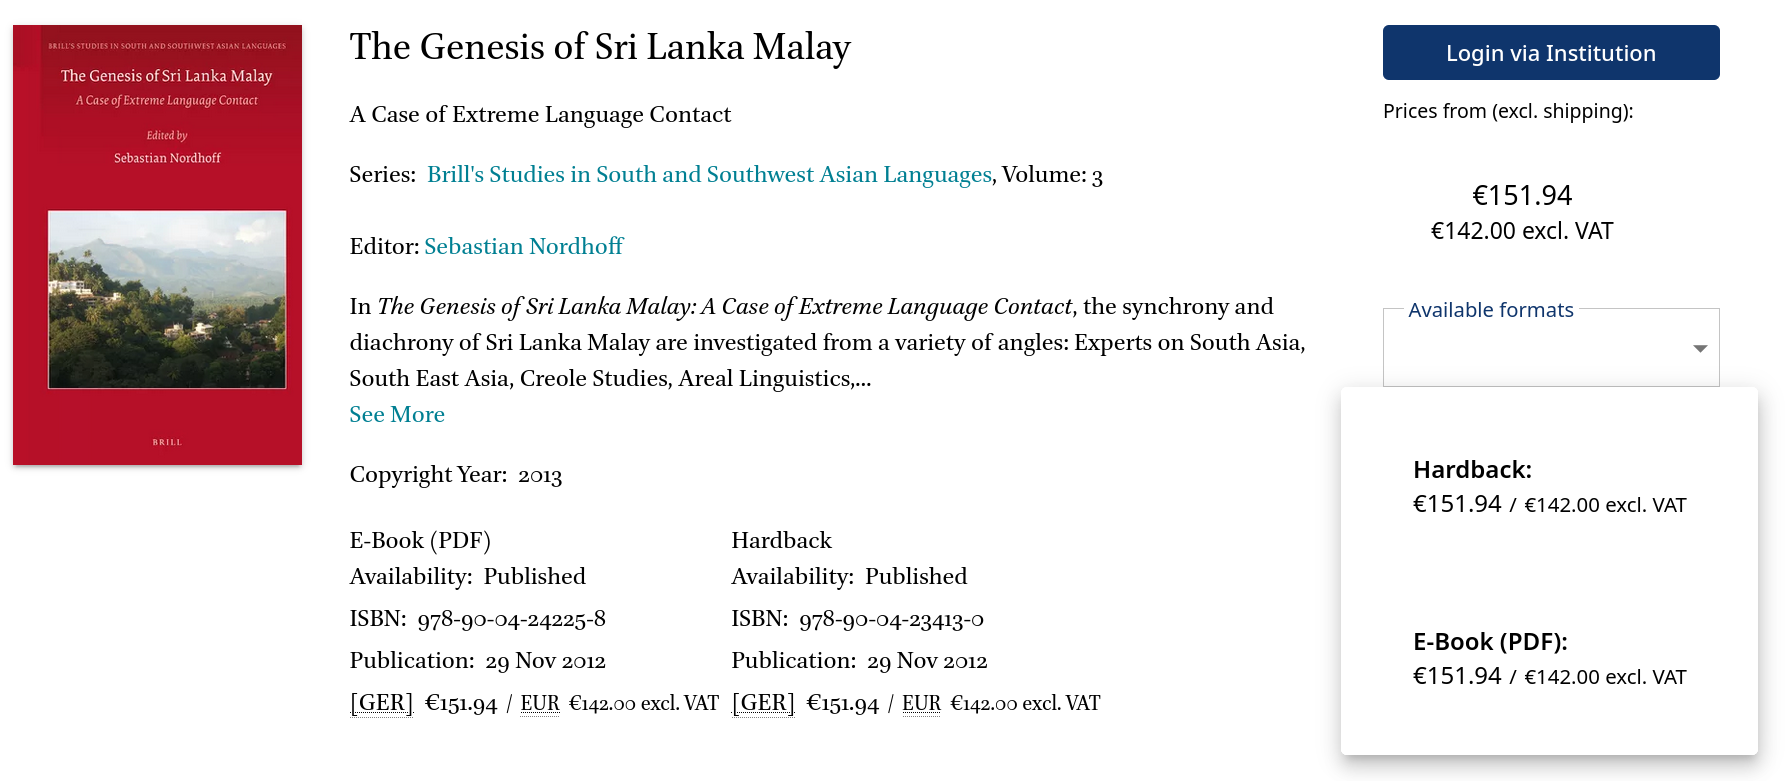
\includegraphics[height=.8\textheight]{brillnordhoff.png}
  \begin{itemize}
    \item  item-based one-off purchase
    \item  institutional bundle 
    \item  patron driven acquisition
  \end{itemize}
}

\frame{
\frametitle{Services provided by\\ publishers}
%   \includegraphics[height=.2\textheight]{./path/to/graphicsfile}
  \begin{itemize}
    \item review facilitation (or not)
    \item  language polishing (or not)
    \item  copy-editing (or not)
    \item  typesetting (or not)
    \item  indexing (or not)
  \end{itemize}
}

\frame{
\frametitle{Funding models: author pays}
%   \includegraphics[height=.2\textheight]{./path/to/graphicsfile}
  \begin{itemize}
    \item  Article processing charges (APCs)
    \item  Book processing charges (BPCs)
    \item Book chapter processing charges (BCPCs)
    \item What is the cost of publishing an article? \pause
    \item What is the cost of publishing a book? \pause
    \item \textit{Scielo} (Brazil) charges 90 USD for one article
    \item \textit{Nature Communications} charges 5200 USD for one article
    \item this explains the profit margins of 30-40\% of the large publishers (Springer, Wiley, Elsevier)
    \item book costs are estimated between 3\,500 and 130\,000 EUR
  \end{itemize}
}

\frame{
\frametitle{Funding model: discipline\\ pays}
%   \includegraphics[height=.2\textheight]{./path/to/graphicsfile}
  \begin{itemize}
    \item institutional funding 
      \begin{itemize}
        \item Uni Bern: \url{https://bop.unibe.ch/linguistik-online}
        \item Uni Hawaii: Journal of Language Documentation and Conservation
      \end{itemize}
    \item learned society funding
      \begin{itemize}
        \item Zeitschrift für Sprachwissenschaft
      \end{itemize}
    \item Subscribe-to-open
      \begin{itemize}
        \item Linguistic Typology
        \end{itemize}
    \item no fees for readers, no fees for authors
    \item host institution covers the costs
  \end{itemize}
}

\frame{
\frametitle{Funding model:\\ decentralized funding}
%   \includegraphics[height=.2\textheight]{./path/to/graphicsfile}
  \begin{itemize}
    \item  Open Library of Humanities (300+ supporting institutions)
    \begin{itemize}
      \item Glossa 
      \item Journal of Portuguese Linguistics 
      \item Laboratory Phonology
      \item Italian Journal of Linguistics 
    \end{itemize}
    \item Language Science Press (100+ supporters)
    \item Open Library Politikwissenschaft (40+ supporting institutions)
  \end{itemize}
}

\frame{
\frametitle{More figures and calculations}
\hfill

\includegraphics[height=\textheight]{cookbook.png}\hfill

\includegraphics[height=\textheight]{businessmodel.png}
\hfill
}

\frame{
\frametitle{Financial aspects:\\ recommendations}
%   \includegraphics[height=.2\textheight]{./path/to/graphicsfile}
  \begin{itemize}
  \highlight
    \item go for discipline-pays
    \begin{itemize}\highlight
    \item else go for author-pays if funds are available 
      \begin{itemize}\highlight
          \item else go for reader-pays and deposit preprints/postprints in repositories. 
      \end{itemize}
    \end{itemize}
  \end{itemize}
}

\section{Sociological aspects}
\frame{
\frametitle{Sociological aspects}
\hspace*{-3cm}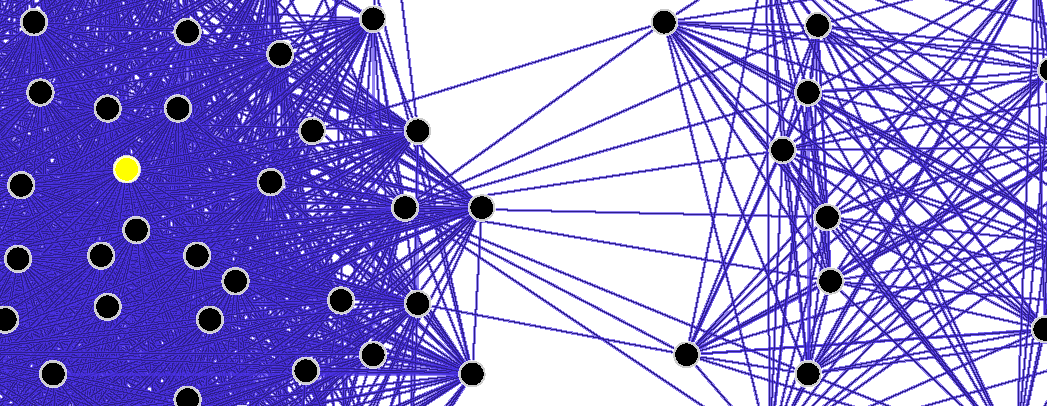
\includegraphics[width=1.6\textwidth]{network.pdf}
}

\frame{
\frametitle{Functions of a publisher}
%   \includegraphics[height=.2\textheight]{./path/to/graphicsfile}
  \begin{enumerate}
    \item  registration \only<2->{$\to$\hfill preprint server} 
    \item   certification \only<3->{$\to$\hfill ???}
    \item   dissemination  \only<4->{$\to$\hfill repository, social media, print-on-demand}
    \item   archiving    \only<5->{$\to$\hfill Zenodo}
  \end{enumerate}
\uncover<6->{The main function which is difficult to substitute remains certification of quality.}
} 

\frame{
\frametitle{Dissemination}
\includegraphics[height=\textheight]{facebook.png}
}

\frame{
\frametitle{Dissemination}
\includegraphics[width=.9\textwidth]{cumulativeall0.png}
}

\frame{
\frametitle{Outsourcing of research\\ evaluation}
%   \includegraphics[height=.2\textheight]{./path/to/graphicsfile}
  
  \parbox{1cm}{~}\begin{itemize}
    \item Universities want to hire good researchers  
    \item The amount of research produced by all candidates combined is too much for the committee to read
    \item The committee use some proxy to judge quality: the brand of the publisher or the journal 
    \begin{itemize}
      \item good publishers, regular publishers, bad publishers, ...
    \end{itemize}
    \item NB: quality selection is done by the (unpaid) editors, not by the publishers
    \item the quality selection process is more or less the same for all publishers
  \end{itemize}
}

\frame{
\frametitle{Brands}
%   \includegraphics[height=.2\textheight]{./path/to/graphicsfile}
  \begin{itemize}
    \item Once a publisher is perceived as prestigious, a self-reinforcing loop starts: 
    \begin{enumerate}
      \item researchers present better manuscripts to the publisher 
      \item the publisher has more material to choose from 
      \item the average quality of the publisher gets better 
      \item prestige goes up
      \item start over 
    \end{enumerate}
    \item Crucially, there is not necessarily more work being done by prestigious publishers 
    \item But since the brand is owned by a company, they increase the prices beyond proportion
  \end{itemize}
}

\frame{
\frametitle{Proofs by a prestigious\\ publisher}
  \includegraphics[width=.6\textwidth]{dg.png}
  ~~~~
  \vspace*{-7cm}\includegraphics[width=.3\textwidth]{semf.png}\vspace*{7cm}  }

\frame{
\frametitle{Errors and Journal Impact Factor}
\includegraphics[width=\textwidth]{jif.png}
\url{biorxiv.org/content/biorxiv/early/2016/08/25/071530.full.pdf}
}  
  
\frame{
\frametitle{It's the employability, stupid}
%   \includegraphics[height=.2\textheight]{./path/to/graphicsfile}
  \begin{itemize}
    \item Being employed as a professor between 40 and 65 years gives you 3\,000\,000 EUR income. 
    \item It is economically rational for each individual researcher to spend 5\,000+ EUR for an article in \textit{Nature} if this improves your chances of becoming a professor
    \item It is economically rational for \textit{Nature} to charge as much as they can since they are a public company
    \item But this sucks money out of research, which could better be used to improve teaching, fund postdocs or develop vaccines. 
    \item Two solutions:
    \begin{itemize}
      \item decouple research evaluation from the place of publication (DORA)
      \item move the brands from the for-profit-sphere to the non-profit-sphere (Fair OA) 
    \end{itemize}
  \end{itemize}
}
%
% \frame{
% \frametitle{Choice of publisher according to JS Caux}
% %   \includegraphics[height=.2\textheight]{./path/to/graphicsfile}
%   \begin{description}
%     \item[\textbf{Gold}] Content is free for readers
%     \item[\textbf{Platinum}] as above, and free for authors
%     \item[\textbf{Palladium}] as above, and all financial statements are disclosed\vspace*{.3cm}\\\pause
%     \item[\textbf{Iron}] pay-to-read\pause
%     \item[\textbf{Lead}] editorial and financial aspects are not hermetically decoupled
%   \end{description}\pause
%   \url{https://jscaux.org/blog/post/2017/09/20/noble-metals-noble-cause/}
%   }


\frame{
\frametitle{Open Access colour codes}
%   \includegraphics[height=.2\textheight]{./path/to/graphicsfile}
  \begin{itemize}
    \item \textbf{green}
    \begin{itemize}
      \item Normal copyrighted publication with a publisher, but copy is archived in an institutional repository
    \end{itemize}
    \item \textbf{gold}
    \begin{itemize}
      \item publication is made openly available against a fee (Article Processing Charge, Book Processing Charge)
    \end{itemize}
    \item \textbf{diamond}
    \begin{itemize}
      \item like Gold OA, but without a fee
    \end{itemize}
      \item (black)
    \begin{itemize}
      \item a copyrighted publication is available via pirate sites/shadow libraries like SciHub or LibGen
    \end{itemize}
    \item (bronze)
    \begin{itemize}
      \item fake open access, not respecting the Berlin Declaration
    \end{itemize}
  \end{itemize}
}


 \frame{
\frametitle{Publisher selection}
%   \includegraphics[height=.2\textheight]{./path/to/graphicsfile}
\begin{itemize}
  \item Fair Open Access Principles (\url{https://www.fairopenaccess.org/the-fair-open-access-principles})
\end{itemize}
\begin{enumerate}
\item    The journal has a \textbf{transparent ownership structure}, and is \textbf{controlled by} and responsive to the \textbf{scholarly community}.
\item     Authors of articles in the journal \textbf{retain copyright}.
\item    All articles are published open access and an \textbf{explicit open access licence} is used.
\item    \textbf{Submission and publication is not conditional} in any way on \textbf{the payment of a fee} from the author or their employing institution, or on membership of an institution or society.
\item    Any \textbf{fees} paid on behalf of the journal to publishers \textbf{are low, transparent, and in proportion} to the work carried out.
\end{enumerate}
}


\frame{
\frametitle{The Green Road:\\ Sherpa Romeo}
%   \includegraphics[height=.2\textheight]{./path/to/graphicsfile}
  \begin{itemize}
    \item Can I deposit my article via the Green Road?
    \item Publisher policies vary
    \begin{itemize}
      \item which version (author submitted version, author accepted manuscript, publisher version)
      \item which embargo period
      \item which repository
    \end{itemize}
    \item Sherpa Romeo is a webservice which gives overviews of different publishers' policies.
    \begin{itemize}
        \item \url{https://v2.sherpa.ac.uk/romeo}
    \end{itemize}
%     \item There is a trick with the Rights Retention Strategy
%     \begin{itemize}
%       \item Before handing in your revised version to the publisher, release it under a Creative Commons license. Then, you  ``re-use'' your own work ``with attribution''. Like that, the copyright does not get transferred.
%     \end{itemize}
  \end{itemize}
}

\frame{
\frametitle{The Golden Road}
%   \includegraphics[height=.2\textheight]{./path/to/graphicsfile}
  \begin{itemize}
    \item Choose your journal
    \item Pay Article processing chargers of 500--3\,000€.
    \begin{itemize}
      \item there might be waivers for people from certain institutions or certain countries
    \end{itemize}
    \item Your article is available as Open  Access
    \item Beware of predatory journals\\\includegraphics[height=2.5cm]{spam.png}
    \item \url{https://thinkchecksubmit.org}
  \end{itemize}
}


\frame{
\frametitle{Directory of Open Access Books (DOAB)}
  \includegraphics[height=\textheight]{doab.png}
  \begin{itemize}
    \item  \url{https://directory.doabooks.org/browse?type=classification_text&value=linguistics}
  \end{itemize}
}



\frame{
\frametitle{Directory of Open Access Journals (DOAJ)}
  \includegraphics[height=\textheight]{doaj.png}
  \begin{itemize}
    \item  \url{https://directory.doabooks.org/browse?type=classification_text&value=linguistics}
  \end{itemize}
}

\frame{
\frametitle{The Diamond Road}
%   \includegraphics[height=.2\textheight]{./path/to/graphicsfile}
  \begin{itemize}
    \item  Choose your journal
    \item Pay 0€
    \item Your article is available as Open Access
    \item \url{oaling.wordpress.com} has a list of Diamond OA journals in linguistics
  \end{itemize}
}

     
     
\frame{
\frametitle{Recommendations for\\ financial aspects}
%   \includegraphics[height=.2\textheight]{./path/to/graphicsfile}
  \begin{itemize}
  \highlight
    \item choose a scholar-led community-owned publisher 
    \item             do not exacerbate libraries' burden
   \item          lobby against stupid criteria of research assesement like the Journal Impact Factor
  \end{itemize}
}



            
% \section{Political aspects}
% \frame{
% \frametitle{Political aspects}
% %   \includegraphics[height=.2\textheight]{./path/to/graphicsfile}
% }

% \frame{
% \frametitle{Political initiatives}
% %   \includegraphics[height=.2\textheight]{./path/to/graphicsfile}
%   \begin{itemize}
%     \item  DEAL: Germany negotiates national OA licensing programmes with big publishers 
%     \item  Plan S: Research funders will require 100\% Open Access from projects they fund 
%     \begin{itemize}
%     \item There are indications that both actions probably lead to an increase in authory-pays publishing fees
%     \end{itemize}
%     \item Sci-Hub and LibGen allow you to access paywalled content and are probably more successful an instrument than all political initiatives 
%   \end{itemize}
% }
% 
% \frame{
% \frametitle{Pollitical miscellanea}
% %   \includegraphics[height=.2\textheight]{./path/to/graphicsfile}
%   \begin{itemize}
%     \item  Swiss National Fund pays generous processing charges 
%     \item Austrian FWF is more on the repository side 
%     \item The San Francisco Declaration on Research Assessment (DORA) calls for a move away from journals/publishers as proxies for research evaluation. 
%   \end{itemize}
% }

       
\frame{
\frametitle{Wrap-up: recommendations\\ \mbox{for sustainable book publications}}
%   \includegraphics[height=.2\textheight]{./path/to/graphicsfile}
  \begin{itemize} 
  \highlight
    \item separate data, code, and text 
    \item use a versioning system
    \item backup\\~
    \item publish all your data in appropriate repositories
    \item use preprint servers\\~
    \item use the CC-0 license for data and the CC-BY license for text
    \item do not sign away your copyright\\~
    \item care for your discipline, go for scholar-led community-owned publishers
  \end{itemize}
}
    
\frame{
\frametitle{Thank you}
  \includegraphics[width=\textwidth]{nebrija.jpg}
}    

\end{document}
